%\documentclass[referee]{aa}
\documentclass{aa}

\usepackage[utf8]{inputenc} 
\usepackage[varg]{txfonts}
\usepackage{amssymb}
\usepackage{epsfig}
\usepackage{graphics}
\usepackage{amsmath}
\usepackage{color}
\usepackage{natbib}
\usepackage{hyperref}
\usepackage{gensymb}
\usepackage{float}

\usepackage{bm}
\usepackage{mathtools}
\usepackage{graphicx}
\usepackage{lipsum}
\usepackage{ulem}


\usepackage{cleveref}

\newcommand{\be}{\begin{equation}}
\newcommand{\ee}{\end{equation}}
\newcommand{\beq}{\begin{eqnarray}}
\newcommand{\eeq}{\end{eqnarray}}
\newcommand{\bc}{\begin{center}}
\newcommand{\ec}{\end{center}}
\newcommand{\unit}[1]{\mbox{\boldmath $\hat{#1}$}}

\newcommand*\df {\mathop{}\!\mathrm{d}}
% \def\beq{\begin{eqnarray}}
% \def\eeq{\end{eqnarray}}
\newcommand{\red}[1]{\textcolor{red}{#1}}
\newcommand{\blue}[1]{\textcolor{blue}{#1}}
\newcommand{\green}[1]{\textcolor{green}{#1}}
\newcommand{\req}{R_{\mathrm{e}}}
\newcommand{\rpol}{R_{\mathrm{p}}}
\newcommand{\ftot}{F^{\mathrm{tot}}}
\newcommand{\fluxp}{F^{\mathrm{p}}}
\newcommand{\fluxs}{F^{\mathrm{s}}}
\newcommand{\msun}{{M}_{\sun}}


%\slugcomment{ }
%\shorttitle{Polarization from neutron stars}
%\shortauthors{Me}

%\voffset=-1cm

\bibpunct{(}{)}{;}{a}{}{,} % to follow the A&A style

%Debug addition for collaborators
%\usepackage[switch, modulo]{lineno}
%\linenumbers
%\renewcommand\linenumberfont{\color{red}\normalfont\tiny\sffamily}
%\renewcommand\linenumberfont{\normalfont\tiny\sffamily}

\DeclareUnicodeCharacter{00A0}{ }

%\slugcomment{ }
%\shorttitle{Polarization from neutron stars}
%\shortauthors{Me}

%\voffset=-1cm

\makeatletter
\def\fvec#1{\underline{\sbox\tw@{$#1$}\dp\tw@\z@\box\tw@}}
\makeatother

\begin{document}
\title{Polarized radiation from rapidly rotating oblate neutron stars}
%new title suggestion:
%\title{Polarized oblate Schwarzschild approximation} %or similar


%\titlerunning{Meme BB}

\author{Vladislav~Loktev\inst{1,2}
\and Tuomo~Salmi\inst{1}
\and Joonas~N\"attil\"a\inst{3,4,5}
\and  Juri~Poutanen\inst{1,2,3}}

\institute{Department of Physics and Astronomy, FI-20014 University of Turku, Finland \\ \email{vladislav.loktev@utu.fi, juri.poutanen@utu.fi}
\and Space Research Institute of the Russian Academy of Sciences, Profsoyuznaya str. 84/32, 117997 Moscow, Russia 
\and Nordita, KTH Royal Institute of Technology and Stockholm University, Roslagstullsbacken 23, SE-10691 Stockholm, Sweden
\and Physics Department and Columbia Astrophysics Laboratory, Columbia University, 538 West 120th Street New York, NY 10027
\and Center for Computational Astrophysics, Flatiron Institute, 162 Fifth Avenue, New York, NY 10010, USA
}

\date{Received XXX / Accepted XXX}




\abstract{
%In this report the radiation escaping a plane-parallel electron consisting neutron star atmosphere is described.
We compute the polarization of radiation from two hotspots at surface of an oblate neutron star (NS) using `oblate Schwarzschild' approximation. 
We account for rotation of the polarization plane due to relativistic effects along the path from the star surface to the observer.
The results are shown to agree with those obtained by performing full numerical general relativistic ray-tracing with the \textsc{arcmancer} code. 
We show that the obtained polarization angle (PA) may differ substantially from the corresponding values derived for a spherical star.
We demonstrate that assuming incorrect shape for the star can lead to biased constraints for NS parameters when fitting the polarization data.
Using a simplified model, we also make a rough estimate of how accurately the geometrical parameters of an accreting NS could be determined using the X-ray polarization measurements of upcoming polarimeters, like \text{Imaging X-ray Polarimeter Explorer} (\text{IXPE}) or \text{enhanced X-ray Timing and Polarimetry} (\text{eXTP}) mission.
%However, this will be investigated in more detail in a follow-up study.
%The results imply that the observer and spot inclination angles can be constrained within a few degrees, if the PA is measured with  accuracy of $2 \degr$ that is achievable  with the upcoming Imaging X-ray Polarimeter Explorer (IXPE) or enhanced X-ray Timing and Polarimetry (eXTP) mission. 
%A&A does not allow italics in the names of satellites except "Rossi" or etc.
%Also the numerical methods for computing flux and polarization degree of outgoing from the star surface radiation are described \blue{(at least not yet described ...)}.
}


\keywords{Polarization  -- stars: neutron -- X-ray binaries -- X-rays: stars}

\maketitle

\section{Introduction}\label{sec:intro}

%general intro
Millisecond pulsars (MSPs) are rapidly rotating neutron stars (NSs) with relatively low magnetic field and many of them are found in binary systems.  
%or something else ...
These NSs are spun up to extreme angular velocities by accretion from its companion (REFERENCES). 
During the accretion phase, matter falls on the NS surface near the magnetic poles creating hotspots that emit polarized X-ray radiation. 
X-ray polarization from accretion-powered millisecond pulsars (AMPs) will be soon measured by the upcoming space observatories, like the \text{Imaging X-ray Polarimeter Explorer} (\text{IXPE}) \citep{IXPE} and the \text{enhanced X-ray Timing and Polarimetry} mission (\text{eXTP}) \citep{EXTP,dmatter_extp}. 
The pulse profiles contain the information about parameters of the NS such as its mass and radius  \citep[e.g.][]{PG03,2016RvMP...88b1001W,SNP18,Bogdanov19L26}. 
The relation between these parameters can give some constraints on the equation of state (EOS) of extremely dense matter constituting the inner parts of a NS \citep[for instance, see][]{lindblom1992,Lattimer12ARNPS}.


%For modelling the pulse profiles from the hotspots of NSs,
%the necessary formalism was first developed by \cite{PFC83}
The core theory on pulse profile modeling was presented in \cite{PFC83} and afterwards extended for rapidly rotating spherical NSs by \citet{PG03} and \citet{PB06} where most of the equations for pulse profile modeling were derived. 
In addition to the modulation of the X-ray flux, \citet{VP04} modeled polarization degree (PD) and polarization position angle (PA) from an infinitely small hotspot (or two antipodal spots) on the surface of rapidly rotating NS. 
\citet{poutanen20} presented a derivation of the formulae used by \citet{VP04} using a so called common vector formalism as well as studied the effect of rapid rotation on the polarization profile. 
From there we also inherit the idea about polarization properties in AMP spectra. 
We get the PD of the hotspot radiation using a relatively simple model of Thomson scattering in a plane-parallel slab \citep[see e.g.][]{ST85,VP04}. 
%Thus we expect that PD changes its sign (and PA switches by 90 degrees) in different parts of the spectrum.
For light bending of rays emitted from the surface of such a compact object we apply Schwarzschild geometry \citep{mtw73,PFC83} and use either a numerical treatment to solve the equations \citep[explained e.g. in][]{SNP18} or the analytical approximation by \citet{poutanen19}.
These approaches have shown to accurately agree each other, although we use the latter method only in Sect.\,\ref{sec:theory}.


%Other effects of fast rotation were also studied by \citet{NP18}, \citet{VBR18}, and \citet{SP20}. % +Braje 2000, Bauböck 2012, Vincent 2018 ? 

Unlike \citet{VP04} and \citet{poutanen20}, we regard a NS that rotates so fast that its shape can no longer be considered spherical. 
The oblate Schwarzschild (OS) approximation was proposed by \citet{CMLC07} and \citet{MLC07} to describe the flux modulation from such stars. 
The corrected formalism in OS \blue{(for non-infitesimal spots?)} case was recently presented by \citet{Bogdanov19L26} and \citet{SP20}, but without considering polarization \red{(But I guess there is no changes from the formalism of \citet{SNP18}?)}. 
In this paper, our aim is to derive analytical expressions for apparent PA for a point source at the oblate surface of rapidly rotating NS.
Then we use these formulae to model pulse profiles and polarization and study the importance of the oblateness effects in such modeling.
According to the NS shape model proposed by \citet{AGM14}, which we also use, polar radius of the NS can differ from equatorial one up to 10\% if the NS rotation rate is close to 600~Hz.
We also allow the emitting hotspots to have measurable sizes.

%more specific intro
% Equation of state (EOS) ...

%history and previous work
% The previous studies ...

%Current problem/gap
% Now we need equations for oblate polarization, since ...

%summary of sections
The remainder of this paper is structured as follows. 
In Sect. \ref{sec:theory}, we present the theory that describes transfer of polarized radiation from one or two hotspots at the surface of an oblate NS to the observer at infinity. 
In Sect.~\ref{sec:results} we first confirm the accuracy of our model by comparing the polarization profiles to those calculated with general relativistic polarized radiative transfer code \citep{PMN18}.
Then we use the theoretical model to fit synthetic PA data in order to estimate how well the NS parameters could be constrained and to see how the results differ if an incorrect shape of the star is assumed.
We conclude in Sect. \ref{sec:conclusions}.
%The results of the modelling are described in Sect. \ref{sec:results}. 
%We discuss the results in Sect. \ref{sec:discussion} and summarize in Sect. \ref{sec:summary}.  


%INSTRUCTED FIGURE FORMATS:
%\begin{figure}
%\resizebox{\hsize}{!}{\includegraphics{<yourfilename.eps>}}
%\caption{<Your caption text...>.}
%%\end{figure}

%%Or for 2-column figure:
%\begin{figure*}
%\centering
%\includegraphics[width=17cm]{<yourfilename.eps>}
%\caption{<Your caption text...>.}
%\label{<Your label>}
%\end{figure*}

\section{Theory}\label{sec:theory}
\subsection{Geometry of the NS}\label{sec:geometry}

%\begin{figure}[H]
%\centering
%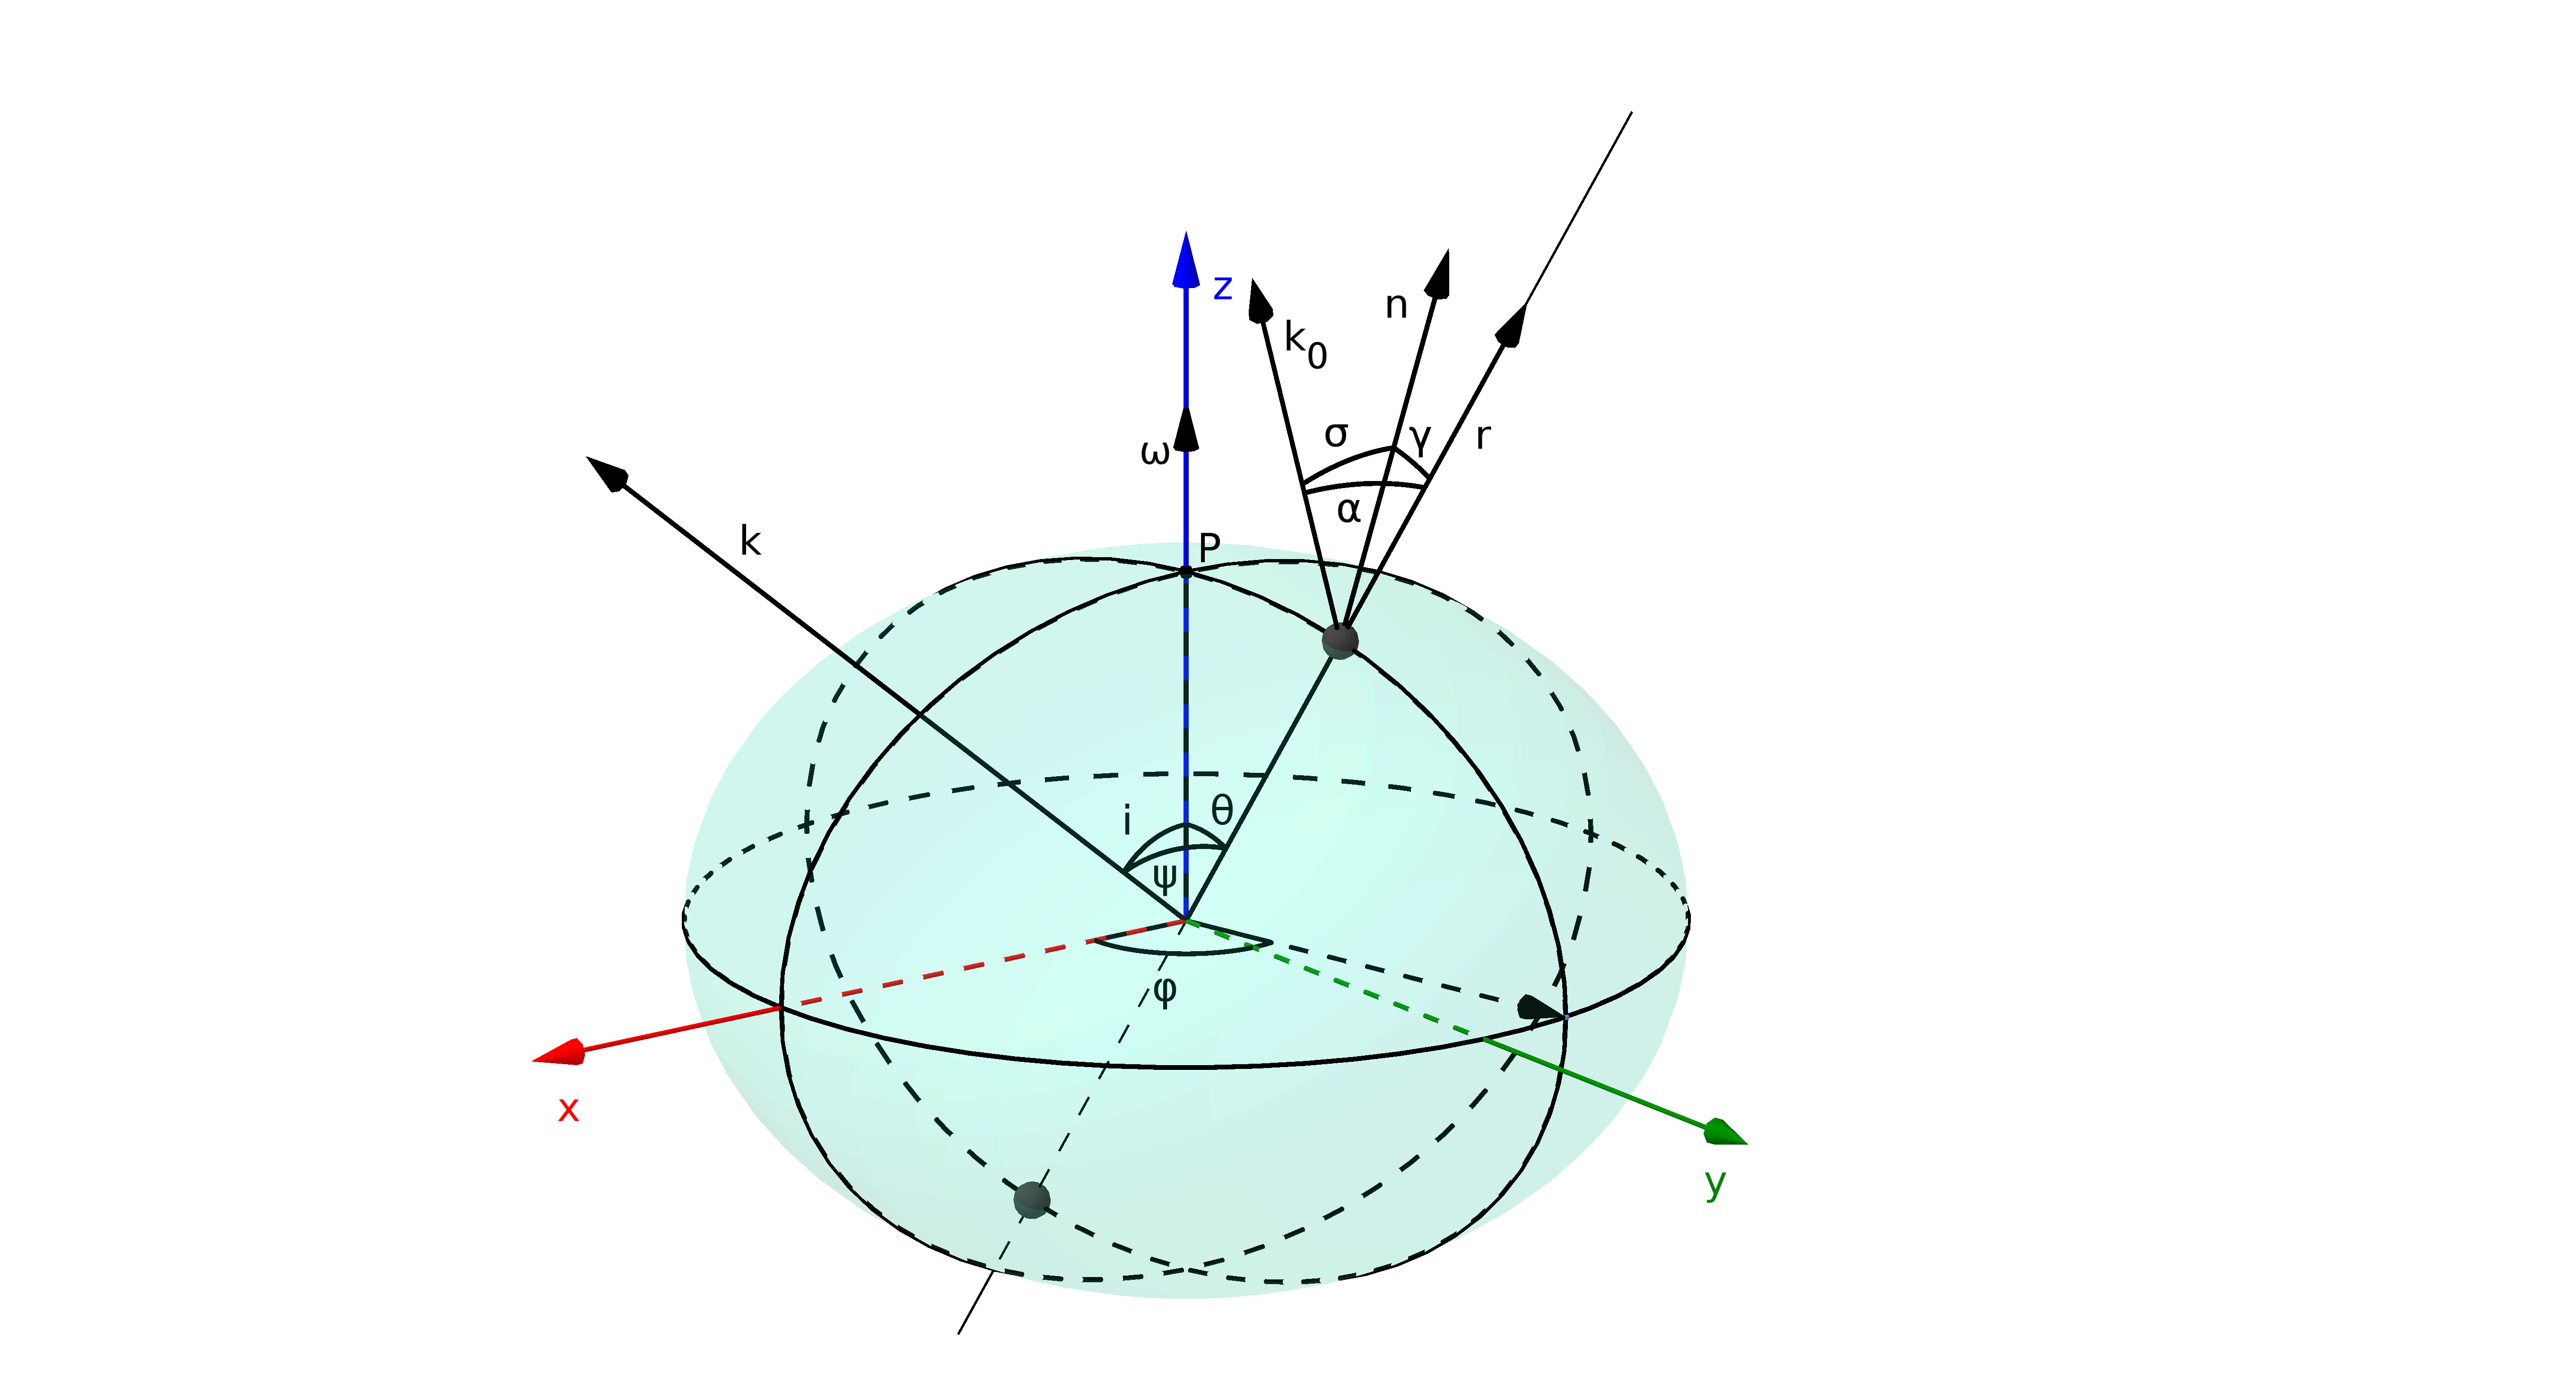
\includegraphics[width=0.7\textwidth]{fig1.png}
%\caption{Geometry of the oblate star. }
%\label{fig:geometry}
%\end{figure}
\begin{figure}
\centering
% \resizebox{\hsize}{!}{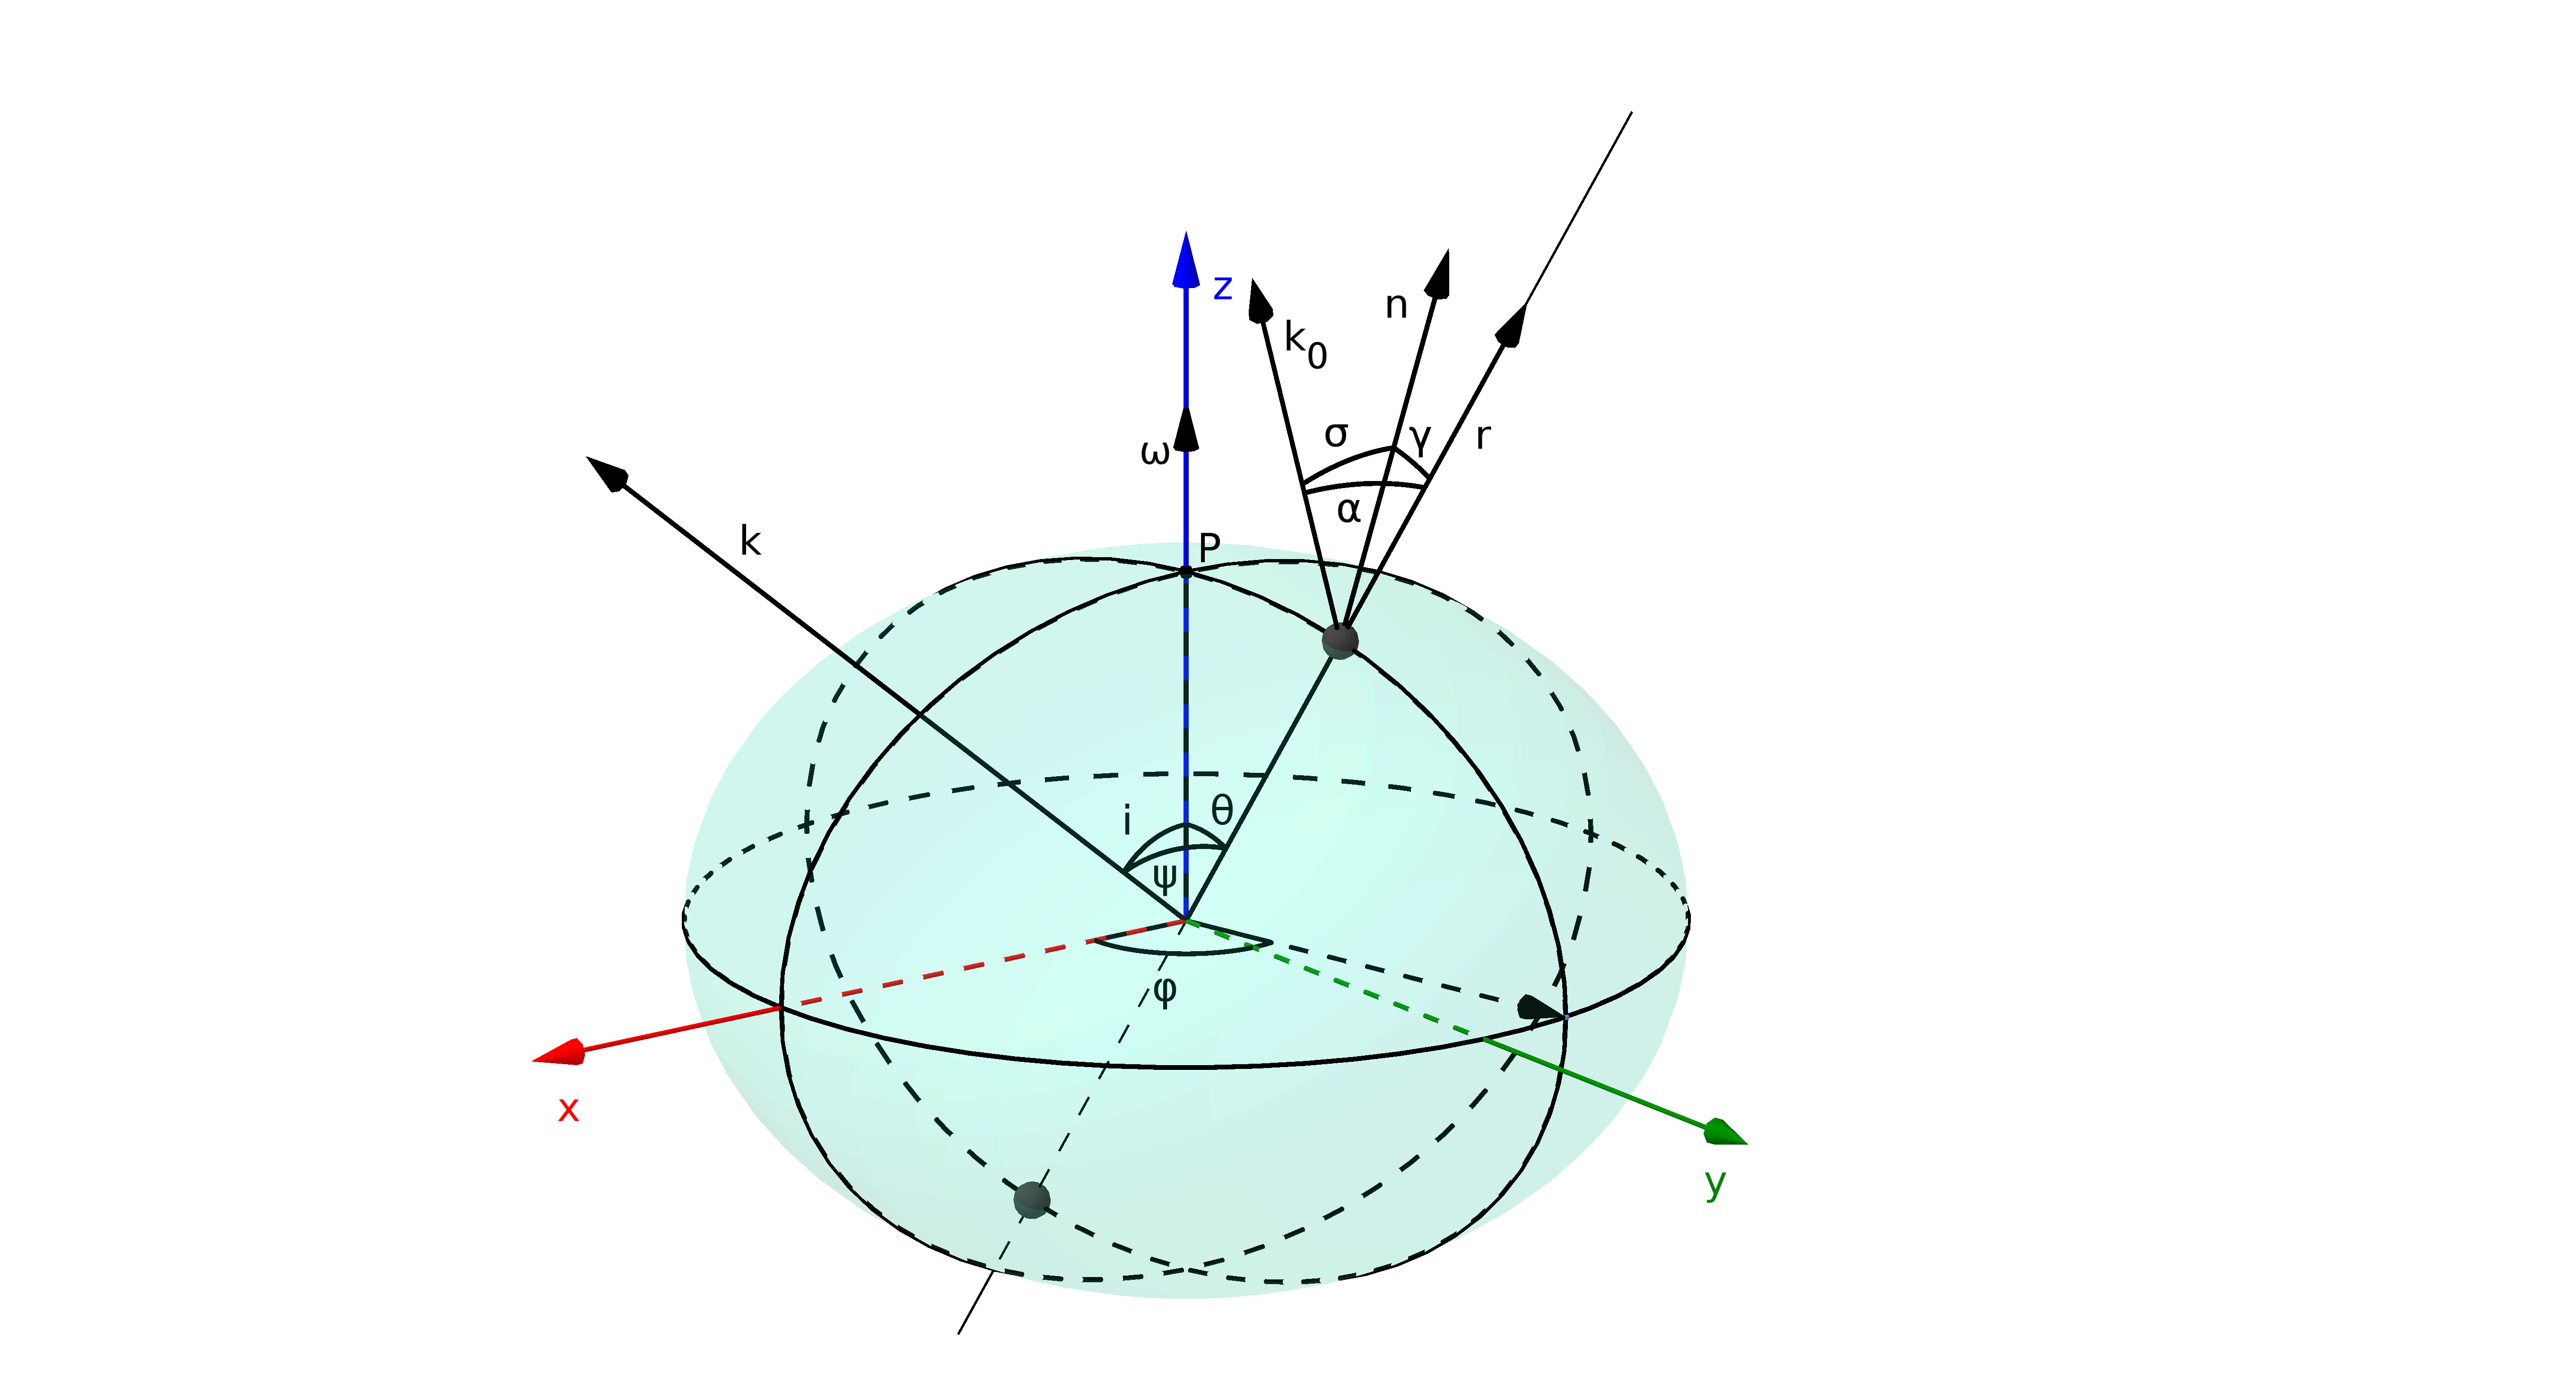
\includegraphics{fig1.png}}
\resizebox{\hsize}{!}{\includegraphics{Geometry.pdf}}
% \resizebox{0.6\textwidth}{!}{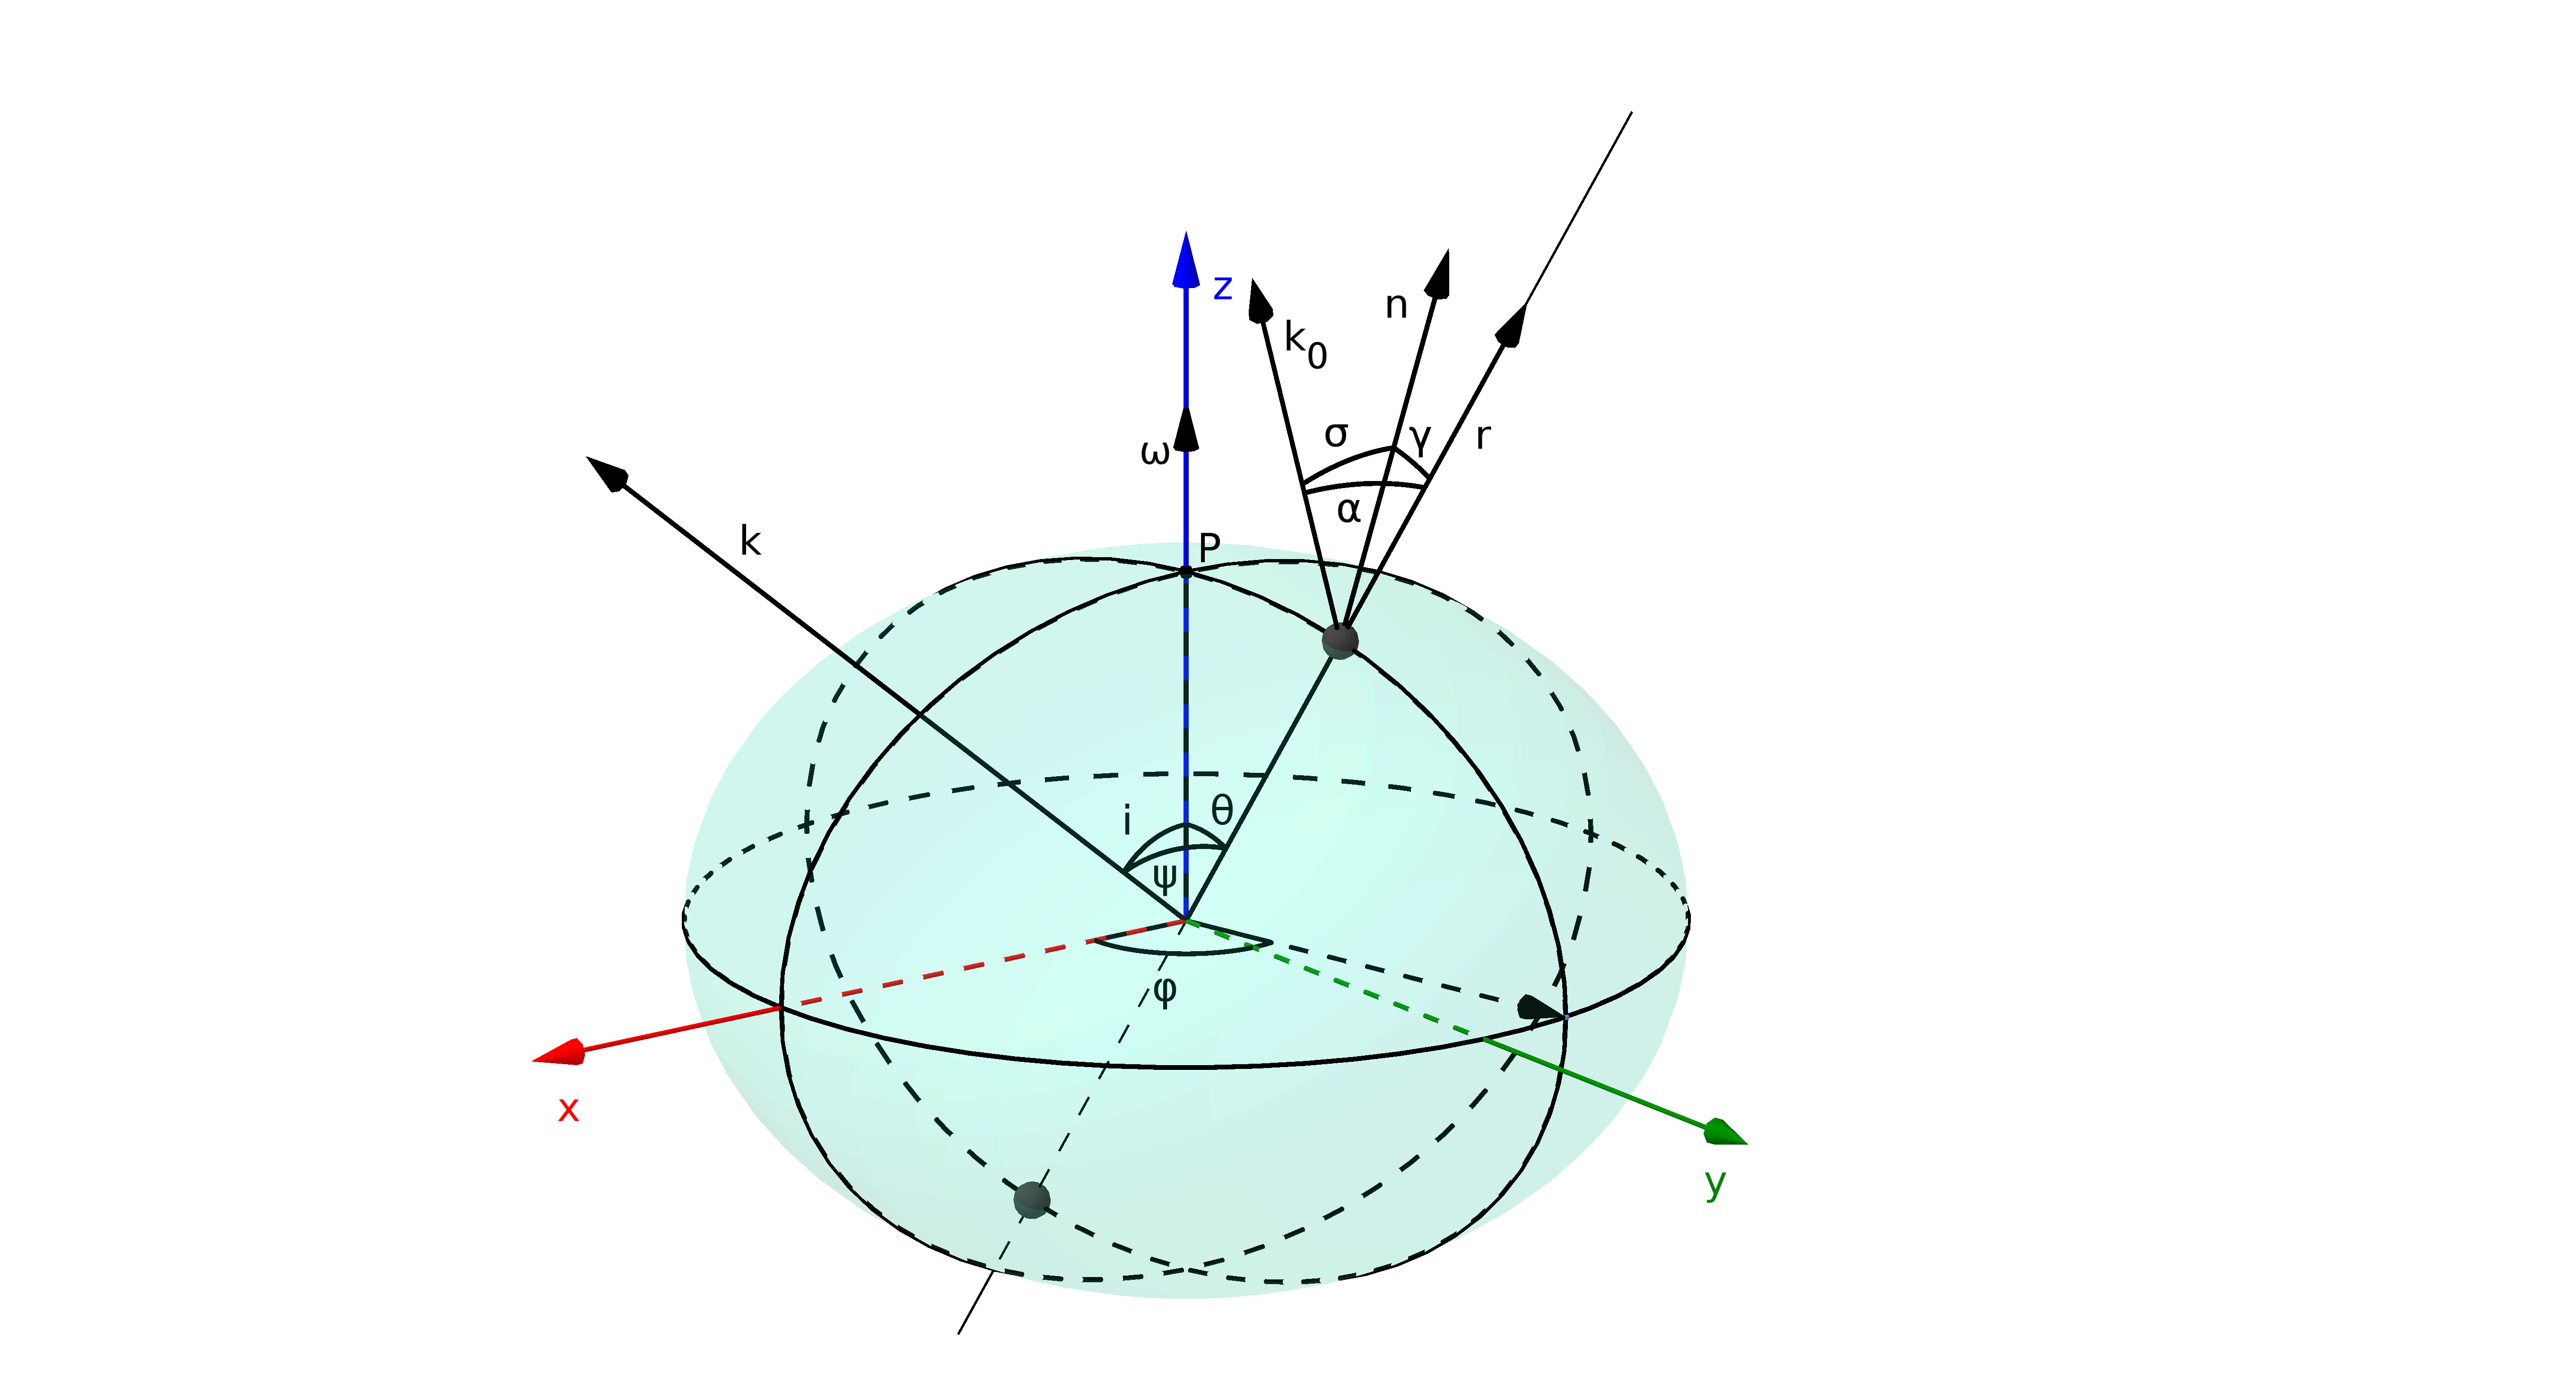
\includegraphics{fig1.png}}
\caption{Geometry of the oblate star and the lab frame coordinate system $\bm{xyz}$. A spot at the NS surface at co-latitude $\theta$ has a rotation phase  $\phi$ from the observer vector $\unit{k}$  around rotational axis  $\bm z$. For the spot three unit vectors are defined: $\unit{n}$ is normal to the surface, $\unit{r}$ is the radius vector and $\unit{k}_0$ is direction of emitted photon propagation.
\red{change $\varphi$ to $\phi$}
}
\label{fig:geometry}
\end{figure}

%https://www.aanda.org/doc\_journal/instructions/aadoc.pdf


We consider a NS of mass $M$ rotating at a high frequency $\nu >300$~Hz, at which the stellar shape flattens significantly \citep{CMLC07,AGM14}. 
The geometry of the star is the same as in \citet{SNP18} and the computation of photon trajectories follows the same methods (except for the comparisons of Sect. \ref{sec:pa_eqs} we apply light bending formula from \citet{poutanen19}).
The axis of pulsar rotation coincides with the symmetry axis, and we choose it to be the applicate axis $\bm z$ in our fixed laboratory frame.  
The direction of the $\bm x$ axis is such that the line of sight to the  observer $\unit{k}$ lies in the plane $\bm{xz}$. 
The $\bm y$ axis completes the right handed Cartesian system.
The unit vector $\unit{k}$ pointing to the direction of the observer from the star center forms angle $i$ with the rotation axis. 

We consider first a small hotspot being placed on the star surface and a constant co-latitude $\theta$. 
For larger spots, we integrate observed Stokes parameters over the spot area. 
%to get the total observed flux and polarization.
The phase of the pulsar $\phi$ is the angle measured counterclockwise around the $\bm z$ axis. 
We define the phase to be zero, when the spot passes through the $\bm{xz}$ plane. 
When we consider more than one spot, we name the closest to the observer as the main, which also defines the phase. 

For every moment of time we define three local unit vectors on the surface related to the spot.
They are the radius vector $\unit{r}$ of the spot, the vector normal to the spot $\unit{n}$, and the vector $\unit{k}_0$ denoting the initial direction of light propagation, emitted so that the photon eventually gets to the observer. 
Correspondingly, we have three angles between these vectors, so that $\gamma$ is between $\unit{n}$ and $\unit{r}$, $\alpha$  is between  $\unit{r}$ and $\unit{k}_0$, and $\sigma$  is between $\unit{n}$ and $\unit{k}_0$.
All mentioned elements are shown in Fig. \ref{fig:geometry}.

Each vector can be represented by a set of coordinates in the lab system. Thus, the radius-vector $\unit{r}$ is 
\be 
\unit{r}=(\sin\theta\cos\phi,\sin\theta\sin\phi,\cos\theta),
\ee
the normal is 
\be 
\unit{n}=(\sin(\theta-\gamma)\cos\phi,\sin(\theta-\gamma)\sin\phi,\cos(\theta-\gamma)),
\ee
and the vector along the line of sight is 
\be
	\unit{k}=(\sin i, 0 , \cos i).
\ee
The vector $\unit{k}_0$ lying between $\unit{r}$ and $\unit{k}$  is expressed as
\be\label{eq:kzero}
	\unit{k}_0=\frac{1}{\sin\psi}\left( \sin\alpha\  \unit{k}+\sin(\psi-\alpha)\ \unit{r}\right) ,  
\ee
where the angle $\psi$ between $\unit{r}$ and $\unit{k}$ is determined by the scalar product of these vectors: 
\be\label{eq:cospsi}
	\cos \psi = \unit{r} \cdot \unit{k} = 
	 \cos i \cos\theta + \sin i \sin\theta\cos\phi 
\ee
and the angle $\alpha$ is related to $\psi$ via the light bending integral \citep{PFC83,B02,SNP18,poutanen19}.

%TS: maybe write here also the formulas for other vectors/angles that were mentioned ...?

The shape of the star is given by the Schwarzschild coordinate $R(\theta)$ which is a function of the co-latitude.
Because the star is rotating, the spot is moving in the lab frame with dimensionless velocity $\bm{\beta}=\unit{\beta}  \beta$,
which we decompose into the product of the unity velocity vector 
\be\label{betahat}
	\unit{\beta} =(-\sin\phi,\cos\phi,0)
\ee
and dimensionless speed in units of speed of light $c$
\be
	\beta=\frac{v}{c} = \frac{2 \pi R(\theta) \sin\theta}{\sqrt{1-r_{\rm s}/R(\theta)}} \frac{\nu}{c},
\ee
where $r_{\rm s}=2GM/c^2$ is the Schwarzschild radius of the NS and we have corrected the observed pulsar frequency for gravitational redshift, which can be expressed as 
\be
	\left(1-\frac{r_{\rm s}}{R(\theta)} \right)^{-1/2}=\frac{1}{\sqrt{1-u}}=1+z.
\ee
The spot speed corresponds to its Lorentz-factor
\be\label{Lorentz-factor}
	\Gamma=\frac1{\sqrt{1-\beta^2}}.
\ee

The vectors $\unit{r}$ and $\unit{n}$ lie in the meridian plane due to the axial symmetry of the star, and the angle $\gamma$ between them depends only on latitude.
The values of trigonometric functions for this angle can be represented as 
\be
\cos\gamma=\frac1{\sqrt{ 1+ f^2(\theta) }}
% \ee
\quad\text{and} \quad
% \be
\sin\gamma=\frac{f(\theta)}{\sqrt{ 1+ f^2(\theta) }},
\ee
where the function $f(\theta)$ can be expressed in terms of function $R(\theta)$ and its derivative
\be\label{eq:shape}
	f(\theta)= \frac{1+z(\theta)}R\frac{\df R}{\df \theta}.
\ee

We use one of the recent rapidly rotating NS shape models presented by \citet{AGM14}.
According to the model, the star shape is given by the approximation 
\be
R(\theta)=\req\left(1+o_2(x,\bar\Omega)\cos^2\theta\right), 
\ee 
where the flattening parameter, which defines the difference between the equatorial radius $\req$ and the polar one $\rpol$,
is given in the first order approximation 
\be
o_2(x,\bar\Omega)=\frac{\rpol-\req}{\req}\approx\bar\Omega^2(1.030x-0.788). 
\ee
Here 
\be
x=\frac{r_{\rm s}}{2\req}
\ee
is the dimensionless compactness parameter and 
\be
\bar\Omega=\Omega\left(\frac{\req^3}{GM}\right)^{\frac12}=2 \pi \nu \left(\frac{\req^3}{GM}\right)^{\frac12}
\ee
is the dimensionless circular rotation frequency. 
% \red{(The definition of $\Omega$ is missing?)} 
This approximation gives the shape of the star with better than 1\% accuracy when $\bar\Omega^2<0.1$, which is fulfilled for  most of the realistic EOS for NSs with $\nu<700$ Hz and $M>M_{\odot}$. 

When comparing results for oblate and spherical stars, we also account for the difference in mass and equatorial radius of the same NS due to its rapid rotation. 
For this purpose, following \citet{SP20}, we relate the gravitational mass $M$ and equatorial radius $\req$ of a rotating NS to the mass $M_0$ and radius $R_0$ of a spherical non-rotating NS of the same baryonic mass:
\be \label{eq:massprime}
M=M_0\left(a_0  + \frac{a_1}{1.1-\bar \nu}+ a_2\,\bar \nu^2\right) 
\ee
and
\be \label{eq:RRe}
 \req =R_0\,\left(0.9766+\frac{0.025}{1.07-\bar \nu}+\,0.07\,M_{1.4}^{3/2}\,\bar \nu^2\right) ,
\ee
where the coefficients are $a_0=1-a_1/1.1$, $a_1=0.001 M_{1.4}^{3/2}$, and $a_2=10 a_1$.
Here $M_{1.4}=M_0/1.4\msun$ and  $\nu_{\rm cr}$ is the critical rotation frequency 
\be \label{eq:critical_nu}
\nu_{\rm cr} = 1278\,M_{1.4}^{1/2}\, \left(\frac{10~{\rm km}}{R_{0}}\right)^{3/2}\ \ \mathrm{Hz}.
\ee

\subsection{Polarization properties} 

\subsubsection{Polarization angle }\label{sec:pa_eqs}

%The instrument observes the polarized radiation in the picture plane.
There are several steps one should make in order to transform the Stokes vector from the co-rotating frame of the star to the sky plane.
Let us first define the main polarization basis, in the sky plane, formed by $\unit{z}$ and $\unit{k}$, 
\be 
\label{eq:mbasis}
\unit{e}_1^{\mathrm{m}} = \frac{\unit{z}-\cos{i} \  \unit{k}}{\sin{i}},\qquad 
\unit{e}_2^{\mathrm{m}} = \frac{\unit{k} \times \unit{z}}{\sin{i}}.
\ee
The vector  $\unit{e}_1^{\mathrm{m}}$ is colinear to the projection of the star rotation axis at the sky plane and the second  vector  $\unit{e}_2^{\mathrm{m}}$ is perpendicular to the first one.
This basis is fixed in the lab frame, because the pulsar rotation  axis (along the $\unit{\omega}$) is very stable and the line of sight (along the  $\unit{k}$) does not change during the observation.
The polarization (pseudo-)vector is observed in this basis.
The PA defines the direction of the polarization vector in a basis, and it is customary to measure it in the counter-clockwise from the first base vector $\unit{e}_1^{\mathrm{m}}$.

\red{JP: I do not understand why we first consider basis formed by $\unit{r}$ and $\unit{k}$ instead of immediately taking the basis $\unit{n}$ and $\unit{k}$? }
\red{TS: Good question. Applying directly $\unit{n}$ and $\unit{k}$ seems to give slightly different angle than $\chi_0+\chi_1$ (eq similar to Eq. \eqref{eq:pa_rvm} but $\theta$ replaced with $\theta-\gamma$). Im not sure which way is correct.}.
Next let us consider the basis formed by $\unit{r}$ and $\unit{k}$:
\be\label{eq:rbasis}
\unit{e}^{\psi}_1 = \frac{\unit{r}-\cos{\psi}\ \unit{k}}{\sin{\psi}},\qquad 
\unit{e}^{\psi}_2 = \frac{\unit{k} \times \unit{r}}{\sin{\psi}}.
\ee
This basis is defined in the same plane as the previous one, as it is also perpendicular to $\unit{k}$. 
However, this basis is rotated relative to the main one.  
The angle between these two bases we denote by $\chi_0$, and
%This angle is measured from the vector of the main basis $\unit{e}_1^{\mathrm{m}}$ in the counter-clockwise direction.
%Using the formula for $\cos\psi$ (see Eq. \eqref{eq:cospsi}), 
the corresponding trigonometric functions are:
\be
\cos{\chi_0}=\unit{e}_1^{\mathrm{m}} \cdot \unit{e}^{\psi}_1 = \frac{\sin{i}\cos{\theta}-\cos{i} \sin{\theta}\cos{\phi}}{\sin{\psi}} , 
\ee \be \label{eq:chi0}
\sin{\chi_0}= - \unit{e}_1^{\mathrm{m}} \cdot \unit{e}^{\psi}_2 = \unit{e}_2^{\mathrm{m}} \cdot \unit{e}^{\psi}_1 = - \frac{\sin{\theta}\sin{\phi}}{\sin{\psi}} ,
\ee
Thus we get the standard expression for the PA of the rotating vector model (RVM) \citep{RC69}:
\be \label{eq:pa_rvm}
\tan\chi_0= \frac{-\sin \theta\ \sin \phi}
{\sin i\ \cos \theta  - \cos i\ \sin \theta\  \cos \phi }.
\ee
For the spherical star and slow rotation that is sufficient, but we have to take into account the relativistic motion and the oblateness of the NS shape.

To take into consideration the surface curvature we define another basis formed by the radius vector $\unit{r}$ and the direction of the light propagation $\unit{k}_0$ near the NS surface,
\be\label{eq:basis}
\unit{e}^{\alpha}_1 = \frac{\unit{r}-\cos{\alpha}\  \unit{k}_0}{\sin{\alpha}},\qquad 
\unit{e}^{\alpha}_2 = \frac{\unit{k}_0 \times \unit{r}}{\sin{\alpha}}=\unit{e}^{\psi}_2.
\ee
This basis describes the plane perpendicular to the initial photon direction close to the NS surface.
Because in Schwarzschild metric the light trajectories are planar, vectors $\unit{e}^{\alpha}_2$ and $\unit{e}^{\psi}_2$ coincide. 
The PA measured in this basis near the surface is the same as that measured by the instrument in the basis denoted by upper index $\psi$ in Eq.\,\eqref{eq:rbasis}, because the polarization vector is parallel-transported along photon trajectory.
In addition we introduce the basis associated with the local normal vector  $\unit{n}$:
\be\label{eq:nbasis}
\unit{e}_1^{\sigma} = \frac{\unit{n}-\cos{\sigma}\  \unit{k}_0}{\sin{\sigma}},\qquad 
\unit{e}_2^{\sigma} = \frac{\unit{k}_0 \times \unit{n}}{\sin{\sigma}} .
\ee
%The last two bases are also lying in the same plane (perpendicular to $\unit{k}_0$). 
This basis is also lying in the same plane as the previous one, perpendicular to $\unit{k}_0$.
The angle between them $\chi_1$ can be computed as
\be
\cos{\chi_1}=\unit{e}_1^{\sigma} \cdot \unit{e}^{\alpha}_1 = \frac{\cos\gamma-\cos\alpha\cos\sigma}{\sin{\alpha}\sin\sigma} , 
\ee
\begin{align}\label{eq:chi1}
\sin{\chi_1} &= \unit{e}^{\alpha}_2 \cdot \unit{e}^{\sigma}_1 = \frac{\unit{n} \cdot (\unit{k}_0\times\unit{r} )}{\sin\alpha\sin\sigma}
= \frac{\unit{k}_0 \cdot (\unit{r}\times\unit{n} )}{\sin\alpha\sin\sigma} \nonumber \\
&= \frac{\sin\alpha}{\sin\psi} \frac{ \unit{k} \cdot (\unit{r}\times\unit{n} )}{\sin\alpha\sin\sigma}
= \frac{ \sin\gamma\sin i \sin\phi}{\sin\psi\sin\sigma}.
\end{align}
If the star is spherical, i.e. $\gamma=0$, this angle is exactly zero.

%The last basis is still connected to the fixed lab frame (instead of co-rotating frame). 
The last step is to take into account the positional vector rotation due to the relativistic motion of the NS surface. 
The relativistic correction of the polarization vector we denote by $\chi'$. 
It can be shown that Lorentz transformation of the first polarization basis vector is \citep[see e. g.][]{NP93} 
% (\red{TS: Do you mean $\unit{e}^{\sigma}_{1}$ or $\unit{e}_{1}$? If the first is true, would it be better to notate the Lorentz transformed basis as $\unit{e}'^{n}_{1}$ or something like that instead of $\unit{e}_{1}'$? If the latter is true, I do not understand why $\chi$' would be calculated using bases $\unit{e}_{1}'$ and $\unit{e}^{\sigma}_{1}$ .}) 
\be\label{eq:primebasis}
\unit{e}_1' = \frac{\unit{n}-\mu (\delta\unit{k}_0-\Gamma\bm{\beta})}{\sqrt{1-\mu^2 } }, %\qquad 
% \unit{e}^{\sigma}_{1}' = \frac{\unit{n}-\mu (\delta\unit{k}_0-\Gamma\bm{\beta})}{\sqrt{1-\mu^2 } }
% \unit{e}_2' = \frac{\bm{k_0'} \times \unit{n}}{\sin{\sigma'}} .
\ee
%\blue{
%(or \cite{VP04} and put 
%$$
%\unit{e}_1' = \frac{\unit{n}-\mu\Gamma (\unit{k}_0-\bm{\beta})}{\sqrt{1-\mu^2 } }
%$$ there would be no difference in the result.)\\}
where  
\be
%	\delta=\frac{1}{\Gamma(1-\bm{\beta}\cdot\unit{k}_0)}
	\delta=\frac{1}{\Gamma(1-\beta \cos\xi)} 
\ee
is the Doppler-factor, $\mu$ denotes the cosine of the inclination of the line-of-sight to the normal in the co-rotating reference frame expressed as  \citep{PG03,PB06}
\be
\mu=\delta\cos{\sigma},  % \equiv\cos\sigma'
\ee
and $\xi$ is the angle between the spot velocity vector and the photon direction  
\be \label{eq:cosxi}
\cos\xi = \unit{\beta} \cdot \unit{k}_0 = -  \frac{\sin\alpha}{\sin\psi} \sin i\ \sin\phi\  .
\ee
 

% \blue{Apparently it is not legit to just apply Lorentz transformation to the vectors in lab basis \eqref{eq:nbasis} and say that we will get the polarization basis in the moving frame. 
% Let letters with primes correspond to values in the co-rotating frame.  Thus, the unit vector of photon propagation is  
% % \be\label{eq:k_0Lorentz}
% $$
% \bm{k_0'}=\unit{k}_0-\Gamma \left(1 -\frac{\Gamma}{\Gamma+1}\bm{\beta}\cdot\unit{k}_0\right) \bm{\beta} , 
% $$
% % \ee
% % \blue{
% or
% $$
% \bm{k_0'}=\Gamma (\unit{k}_0-\beta)+\frac{\Gamma-1}{\beta^2}\beta\times(\beta\times\unit{k}_0)
% $$
% and it could be normalized to unity by $\delta$. 
% In the proper expression \eqref{eq:primebasis} for a base vector we have just 
% % which is a unity vector. In VP04 it looked like the vector 
% $$
% \Gamma (\unit{k}_0-\beta)
% $$
% and one can see, that the term $$ \frac{\Gamma^2}{\Gamma+1}\beta\times(\beta\times\unit{k}_0)
% $$ would give a error of order $\beta^2$ to the result. }

This implies that the expressions for the trigonometric functions of the polarization plane relativistic rotation are as follows. 
The sine of the angle $\chi'$ is
\begin{align}\label{eq:sinchi}
\sin{\chi'}&=\unit{e}_1'\cdot \unit{e}_2^{\sigma} =
\frac{\mu\Gamma\beta}{\sin{\sigma}\sqrt{1-\mu^2} } \unit{\beta} \cdot(\unit{k}_0 \times \unit{n}) \nonumber
\\
&=\frac{\beta\cos\sigma }{\sin{\sigma}\sqrt{1-\mu^2}  (1-\beta\cos\xi)} \unit{\beta} \cdot(\unit{k}_0 \times \unit{n}).
\end{align}
			
% % % %  probably doesn't need to be shown

% The scalar triple product $\unit{\beta} \cdot(\unit{k}_0 \times \unit{n})$ %, in Eq. \eqref{eq:sinchi} 
% can by expressed as
% \begin{align}\label{eq:tripleproductoblate}
% \unit{k}_0 \cdot (\unit{n}\times\unit{\beta} )&=
% \unit{k}_0 \cdot \left(\unit{n} \times \frac{\unit{n} \times \unit{r}}{\sin{\gamma}}\right)=
% \unit{k}_0 \cdot \frac{\cos{\gamma}\unit{n} - \unit{r}}{\sin{\gamma}} \nonumber \\
% &=\frac{\cos{\sigma}\cos{\gamma}-\cos{\alpha}}{\sin{\gamma}}.
% \end{align}
% % no $\pm$ sign now 
% Then we get
% \be\label{eq:chiprime}
% \sin{\chi'}=\unit{e}_1'\cdot \unit{e}_2^{\sigma} =
% \frac{\mu\Gamma\beta (\cos{\sigma}\cos{\gamma}-\cos{\alpha})}{\sin{\gamma}\sin{\sigma}\sqrt{1-\mu^2} }.
% \ee

The vector product $\unit{k}_0 \times \unit{n}$ is essentially %, in Eq. \eqref{eq:sinchi} 
% To make another expression, usable more generally, let us then  consider 
the meridional vector headed towards the north pole \red{JP: it is certainly not!}
\be
\unit{m} = (- \cos \lambda \cos \phi, -\cos \lambda \sin \phi, \sin \lambda ),
\ee
where $\lambda \equiv \theta-\gamma$ is the angle between the normal vector and the spin axis, and let $\zeta$ be the angle that the meridional makes with the vector $\unit{k}$
\begin{equation}\label{eq:zeta_defined}
\cos \zeta = \unit{m} \cdot \unit{k} = \cos i \sin \lambda - \sin i \cos \lambda \cos \phi.
\end{equation}
Then using Eq. \eqref{eq:kzero} we can express the scalar triple product  % $\bm{\hat\beta} \cdot(\unit{k}_0 \times \unit{n})$ 
from  Eq. \eqref{eq:sinchi}  as
\begin{align}\label{eq:tripleproductpherical}
\unit{k}_0 \cdot (\unit{n}\times\unit{\beta} )&=\unit{k}_0 \cdot \unit{m} 
= \frac1{\sin\psi}(\sin \alpha \cos \zeta - \sin(\psi-\alpha)\sin\gamma ) \nonumber	\\
&= (\cos\zeta+\cos\psi \sin\gamma)\frac{\sin\alpha}{\sin\psi} - \cos \alpha\sin\gamma.
\end{align}
% and we can use small and even zero $\gamma$ angle.
% * <belliavesha@gmail.com> 2018-05-09T16:50:03.258Z:
%
% ^.
For the small enough $\psi$ angles we may make use of Beloborodov's approximation \citep{B02} or the improved version of it by \citet{poutanen19}. 
The universal formula for the $\sin\chi'$ is then 
% \be\label{eq:sinchiprime}
% \sin\chi'={\mu\beta(1 - a_0) }\frac{(\cos\zeta+\cos\psi \sin\gamma)\frac{\sin\alpha}{\sin\psi} - \cos \alpha\sin\gamma}{\sin{\sigma}\sqrt{1-\mu^2}  (1-\bm \beta \cdot \unit{k}_0)}.
% \ee  
\be\label{eq:sinchiprime}
\sin\chi'={\beta \cos\sigma }
\frac{
\cos\zeta \sin\alpha+\sin(\alpha-\psi) \sin\gamma}
{\sin\psi\sin{\sigma}\sqrt{1-\mu^2}  (1-\bm \beta \cdot \unit{k}_0) }.
\ee  
In particular, for the spherical star we have the result 
\be\label{eq:chiprimespherical}
\sin{\chi'} =
\beta \cos\sigma \frac{\cos i \sin \theta - \sin i \cos \theta \cos \phi}{\sin{\psi}\sqrt{1-\mu^2} (1-\bm \beta \cdot \unit{k}_0)}.
\ee
The cosine of this angle is obviously always positive and one may use the Pythagorean trigonometric identity, but in case of $\sigma\approx0$ or $ \sigma'\approx0$ it will also be useful to have a direct formula 
\begin{align}
\cos\chi'&=\unit{e}_1'\cdot \unit{e}_1^{\sigma} =
% \frac{\unit{n}-\mu \Gamma\left(\unit{k}_0-\bm{\beta} \right)}{\sqrt{1-\mu^2 } }
% \cdot 
% \frac{\unit{n} - \cos \sigma  \unit{k}_0 }{\sin{\sigma}} \nonumber  \\
% &=
\frac{1-\cos^2\sigma- \delta  \Gamma \cos^2 \sigma   \bm \beta \cdot \unit{k}_0 }{\sin{\sigma}\sqrt{1-\mu^2} } \nonumber  \\
% &= \frac{\sin^2\sigma- \Gamma \mu^2  (1 - a_0) \bm \beta \cdot \unit{k}_0 }{\sin{\sigma}\sqrt{1-\mu^2} }
% &=\frac{\sin^2\sigma-  \cos^2 \sigma \bm \beta \cdot \unit{k}_0 /(1-\bm \beta \cdot \unit{k}_0) }{\sin{\sigma}\sqrt{1-\mu^2} }  \nonumber  \\ 
% &=\frac{\sin^2\sigma -\bm \beta \cdot \unit{k}_0 \sin^2\sigma - \cos^2 \sigma \bm \beta \cdot \unit{k}_0 }{\sin{\sigma}\sqrt{1-\mu^2} (1-\bm \beta \cdot \unit{k}_0) } \nonumber  \\
&=\frac{\sin^2\sigma -\bm \beta \cdot \unit{k}_0 }{\sin{\sigma}\sqrt{1-\mu^2} (1-\bm \beta \cdot \unit{k}_0) }. 
% \nonumber  \\
% &=\frac{\sin^2\sigma + \beta \frac{\sin \alpha }{\sin\psi} \sin i \sin \phi (1 - a_0\cos^2 \sigma )}{\sin{\sigma}\sqrt{1-\mu^2} (1+ \beta \frac{\sin \alpha }{\sin\psi} \sin i \sin \phi) }  
\label{eq:coschiprime}
\end{align}	

Combing Eqs.~\eqref{eq:cosxi}, \eqref{eq:sinchiprime} and \eqref{eq:coschiprime} we get 
\be\label{eq:chiprime}
\tan\chi' = \beta \cos \sigma\frac{\cos\zeta + \sin \gamma  \frac{\sin (\alpha-\psi)}{\sin \alpha}}{\frac{\sin \psi}{\sin \alpha}\sin^{2}\sigma + \beta \sin i \sin \phi}.
\ee
% \be\label{eq:chiprime}
% \tan\chi' = \frac{\cos\zeta + \sin \gamma (\cos \psi - \frac{\sin \psi}{\sin \alpha}\cos \alpha)}{\frac{\sin \psi}{\sin \alpha}\frac{\sin^{2}\sigma}{\mu\beta\Gamma\delta(1-
% % \frac{\Gamma-1}{\Gamma\beta^2}\bm{\beta}\cdot\unit{k}_0
% a_0
% )} +  \sin i \sin \phi\cos\sigma }.
% \ee
For the case of a spherical star we put $\gamma=0$ and get a similar expression
\be\label{eq:chiprime_sphere}
\tan\chi'_{\mathrm{sph}} = \beta 
% \red{\delta}
\cos \alpha \frac{\cos i \sin \theta - \sin i \cos \theta \cos \phi}{\sin \psi\sin\alpha + \beta \sin i \sin \phi
% \red{(1+(\delta-1)\cos^2\sigma)}
},
\ee
which coincides with Eq. (29) from \citet{VP04} and derived by \citet{poutanen20}.


The total PA for each spot is then obtained by summing the angles between intermediate bases, since they are constant for parallel transport along the photon trajectory: 
\be\label{eq:chi_tot}
\chi_{\mathrm{obl}}=\chi_0+\chi_1+ \chi'.
\ee
Similarly, for the spherical case this reads
\be\label{eq:chi_tot_sph}
\chi_{\mathrm{sph}}=\chi_0+\chi'_{\mathrm{sph}}.
\ee
We compare the analytic expressions for the angles in Eqs.\,\eqref{eq:chi_tot} and \eqref{eq:chi_tot_sph} in Figs.~\ref{fig:diff_theta}--\ref{fig:diff_nu}, for different co-latitudes, inclinations, and spin frequencies.
For the spherical star we take fix the radius as $R_0=12$\,km and $M_0=1.4\msun$. 
For the oblate star, we compute gravitating mass and equatorial radius using  Eqs.\,\eqref{eq:RRe} -- \eqref{eq:massprime}.
At a spin rate of $\nu = 600$ Hz, the angle $\gamma$ can be as large as $7\degr$ at $\theta = 45\degr$.
Therefore in Figs.~\ref{fig:diff_theta} and \ref{fig:diff_incl} for some curves the condition of $\theta-\gamma < i$ is satisfied whereas for other $\theta>i$. 
In those situations the dashed and solid lines (for spherical and oblate stars, respectively) have opposite monotonicities and large deviation in the vicinity of $\phi=0$. 
\red{it seems that the PA are plotted as a function of emission phase $\phi$, not 
the observed phase, while for spherical and oblate star time delays are different}
\red{(TS: I guess we could account for the time delay as well.)}
However, we note that the PD (see next Section) is expected to be smallest during the same phase (since the spot normal is pointing towards the observer), and thus such high difference between spherical and oblate star may still be difficult to observe.
In addition, from Fig. \ref{fig:diff_nu} we see that the deviation becomes smaller with decreasing spin frequency, as expected.


% \begin{figure}
% \resizebox{\hsize}{!}{\includegraphics{pa_eq_all.pdf}}
%     \caption{
% Comparison of polarization angles $\chi$ (magenta solid line), $\chi_{0}$ (green solid line), $\chi_{1}$ (black solid line), and $\chi'$ (blue solid line) for an oblate NS with $\nu = 600$ Hz, $\req = 12$~km, $M = 1.4~\msun$, $\theta = 60\degr$, $i = 40\degr$. 
% The corresponding results for spherical star are shown by magenta dashed (for $\chi$) and red solid line (for $\chi'_{\mathrm{sph}}$).
% Angle $\chi_{1}$ is zero for a spherical star and $\chi_{0}$ is same for both oblate and spherical stars.
%     }
%     \label{fig:paeq_all}
% \end{figure}
% \begin{figure}
% \resizebox{\hsize}{!}{\includegraphics{pa_eq_freq.pdf}}
%     \caption{
% Comparison of polarization angles $\chi_{1}$ (black lines for oblate star) and $\chi'$ (blue lines for oblate and red for spherical star) for $\nu = 600 $ Hz (solid lines) and $\nu = 300$ Hz (dashed lines).
% Otherwise the parameters and the symbols are the same as in Fig \ref{fig:paeq_all}.
%     }
%     \label{fig:paeq_freq}
% \end{figure}
% \begin{figure}
% \resizebox{\hsize}{!}{\includegraphics{pa_eq_angles.pdf}}
%     \caption{
% Comparison of polarization angles $\chi_{1}$ (black lines for oblate star) and $\chi'$ (blue lines for oblate and red for spherical star) for different angles $i$ and $\theta$.
% Solid lines show the model for $i=40\degr$ and $\theta=60\degr$.
% Dashed lines show the model for $i=60\degr$ and $\theta=40\degr$.
% Dot-dashed lines show the model for $i=80\degr$ and $\theta=20\degr$.
% Other parameters and symbols are the same as in Fig. \ref{fig:paeq_all}. \ref{fig:paeq_all}.
%     }
%     \label{fig:paeq_angles}
% \end{figure}



\begin{figure}
\resizebox{\hsize}{!}{\includegraphics{fig2c.pdf}}
\caption{\textit{Upper panel}: Polarization angles computed for spherical (dashed) and oblate (solid) cases depending on the rotation phase $\phi$ for different co-latitudes of the spot  $\theta$=15\degr\ (red), 30\degr\ (green), 45\degr\ (blue), and 60\degr\ (purple). 
\textit{Lower panel}: The difference between PA for oblate and spherical cases. 
Parameters of a non-rotating NS are $R_0 = 12$~km and $M_0 = 1.4~\msun$, while in the oblate case of a NS rotating at a rate of $\nu = 600$ Hz, the mass and radius are computed according to Eqs.~\eqref{eq:RRe} and \eqref{eq:massprime}. 
The inclination is $i = 40\degr$.
}
\label{fig:diff_theta}
\end{figure}

\begin{figure}
\resizebox{\hsize}{!}{\includegraphics{fig3c.pdf}}
\caption{Same as Fig.~\ref{fig:diff_theta}, but for different inclinations $i$=15\degr\ (red), 30\degr\ (green), 45\degr\ (blue), and 60\degr\ (purple).  
Here the spot  co-latitude $\theta = 35\degr$.}
\label{fig:diff_incl}
\end{figure}

\begin{figure}
\resizebox{\hsize}{!}{\includegraphics{fig4c.pdf}}
\caption{Same as Fig.~\ref{fig:diff_theta}, but for different frequencies $\nu = 1$  (red),  200 (green), 400 (blue), and 600~Hz (purple).
Here the spot co-latitude is $\theta = 40\degr$ and inclination is $i=50\degr$. }
    \label{fig:diff_nu}
\end{figure}


\subsubsection{Polarization degree}

Since we do not consider circular polarization, the Stokes vector contains three components $(F_I,F_Q,F_U)$.
In the last polarization basis (in the co-moving frame of the spot), the polarization angle will always equal to zero, because of axial symmetry of the neutron star, and then $F_U$ will be also always zero. Polarization degree $P$ in this case is determined by  $F_Q=P F_I$, and will not change if the polarization basis rotates. When we rotate the Stokes vector to the main basis, we get the vector 
\be
(F_I, F_Q \cos{2\chi},F_Q \sin{2\chi})
\ee
as a result.

The total Stokes vector is obtained from summing the vectors for primary and secondary spots (denoted by indexes $\mathrm{tot}$, $\mathrm{p}$ and $\mathrm{s}$ respectively) if there are two spots on the NS, and when the spots have a finite size (assuming circular shapes), we integrate over their area using Gaussian quadratures \blue{in magnetic co-latitude (i.e. the angle measured from the magnetic pole) and the corresponding azimuth.} \red{(TS: As Vlad mentioned earlier, this method may not be very good, but at least we used such high resolution in these angles that pulse profiles matched to those computed same way as in Salmi et al. 2018. Secondly, I guess it is not very exact to express the integral like this since the flux from every sub-spot is also multiplied with the corresponding weight. Maybe just remove or little modify the next Eqs)}:
\begin{align}
\ftot_I=\fluxp_I+\fluxs_I = \sum_i F_I^{\mathrm{p},i}+F_I^{\mathrm{s},i}, \nonumber \\
\ftot_Q=\fluxp_Q+\fluxs_Q = \sum_i F_Q^{\mathrm{p},i}+F_Q^{\mathrm{s},i} ,  \\
\ftot_U=\fluxp_U+\fluxs_U= \sum_i F_U^{\mathrm{p},i}+F_U^{\mathrm{s},i}  . \nonumber
\end{align}
% For the integration over spot we use a method, where ... \blue{(which is at least not yet the same as in the paper \citet{SNP18})} ... or is it?
The degree of polarization is then
\be
P^{\mathrm{tot}}=\frac{\sqrt{(\ftot_Q)^2+(\ftot_U)^2}}{\ftot_I},
\ee
and the polarization angle \blue{$\chi^{\mathrm{tot}}$ can be computed from }
\be
%\tan{2\chi^{\mathrm{tot}}}=\frac{\ftot_U}{\ftot_Q}.
\sin{2\chi^{\mathrm{tot}}}=\frac{\ftot_Q}{\ftot_I}, \qquad 
\cos{2\chi^{\mathrm{tot}}}=\frac{\ftot_U}{\ftot_I}.
\ee
%\blue{TS: Maybe still a stupid question, but how can you solve $\chi^{\mathrm{tot}}$ from here, if you don't know the correct quadrant of the angle. Apparently you can assume that $\sin 2\chi^{\mathrm{tot}} = \ftot_U$ and $\cos 2\chi^{\mathrm{tot}} = \ftot_Q$? But I do not see equivalence between these two conditions and eq. (41).}
%\blue{JP: e.g. you can use atan2 routine (in fortran) with two arguments, i.e. you actually know the quadrant.}
%\red{TS: So the correct quadrant is just our choice? We could as well solve $2\chi^{\mathrm{tot}} = \mathrm{atan}(\ftot_U /\ftot_Q) = \mathrm{atan}(-\ftot_U /-\ftot_Q)$, and get different angles depending whether we use $\mathrm{atan2}(\ftot_U ,\ftot_Q)$ or $\mathrm{atan2}(-\ftot_U ,-\ftot_Q)$?}

%In any case, we have still considered only infinitesimally small spots, in order to make more simplified comparisons between polarization from oblate and spherical stars.

\subsection{Intensity and polarization}\label{sec:thomson_atm}

%\blue{TS: I guess repeating all the equations of VP04 is not necessary here. I just tried to summarize the method with words. Please, check for my mistakes or if I missed something.}

As seen in the previous section, we need to calculate the components of the local Stokes vector, in order to get the total polarization angle.
The intensity and polarization of radiation emerging from the emission region depend on both emission angle and energy, and therefore we need also a spectral model. 
We calculate the intensities using the same plane-parallel slab model for the accretion shock as \citet{VP04}  \citep[see also][]{ST85}, which assumes Thomson scattering and corresponding polarization.
Unpolarized seed soft photons are assumed to be injected from the bottom of the slab and then scattered $n$ times before escaping.
Using the procedure of \citet{VP04}, we compute spectra for plenty of scattering orders, and get the final spectrum as a sum of intensities for different scattering orders.
When calculating the pulse and polarization profiles, we interpolate the spectral tables, computed in advance, to match the corresponding emission angle and energy.

The Thomson model, that is used here, is only approximative for accretion-powered millisecond pulsars. 
As a next step, one should make use of the more exact formalism for Compton scattering in a hot slab \citep[see e.g.][]{PS96}.
However, since the focus of this article is on the geometry of star and on the effects of oblateness to the polarization angle, the choice of the spectral model is not very important in this case. 
In practice, the total polarization angle $\chi^{\mathrm{tot}}$ is almost independent of the photon energy.
The only major difference is a $90 \degr$ rotation in $\chi^{\mathrm{tot}}$ when the polarization degree changes its sign as function of energy.

\iffalse 
\subsubsection{Thomson scattering}
The intensity of unscattered photons is
\begin{equation}
I_{l,r}^0=I_{in}e^{-\tau/\mu}
\end{equation} The boundary conditions for $n$ times scattered photons are
\be
I_{l,r}^n(\tau=0,\mu)=I_{l,r}^n(\tau=\tau_T,-\mu)=0\qquad (0\leq\mu\leq1)
\ee
The intensity of $n$ times scattered photons are computed from
\begin{align}
I_l^n(\tau,\mu)&=\int_{\tau_b(\mu)}^\tau \frac{d\tau'}\mu e^{\frac{\tau'-\tau}\mu}
\left( A^n(\tau')(1-\mu^2) + (B^n(\tau')+C^n(\tau')\mu^2 \right),\nonumber\\
I_r^n(\tau,\mu)&=\int_{\tau_b(\mu)}^\tau \frac{d\tau'}\mu e^{\frac{\tau'-\tau}\mu}
\left(B^n(\tau')+C^n(\tau')\right),
\end{align}
where 
\begin{align}
A^n(\tau)&=\frac34\int_0^1 d\mu' (I^{n-1}_l (\tau,\mu')+I^{n-1}_l (\tau,-\mu')) (1-\mu'^2) \nonumber\\
B^n(\tau)&=\frac38\int_0^1 d\mu' (I^{n-1}_l (\tau,\mu')+I^{n-1}_r (\tau,-\mu'))\mu'^2 \\
C^n(\tau)&=\frac38\int_0^1 d\mu' (I^{n-1}_r (\tau,\mu')+I^{n-1}_r (\tau,-\mu')) \nonumber
\end{align}

Then one can compute the intensity of escaping photons\be
I(\mu)=I_l(\tau_T,\mu)+I_r(\tau_T,\mu)
\ee
and the polarization degree of the outgoing radiation (see Figure \ref{figure:ThomsonIp})
\be
p(x,\mu)
=\frac{I_l(\tau_T,\mu)+I_r(\tau_T,\mu)}{I_l(\tau_T,\mu)-I_r(\tau_T,\mu)}
=100\%\frac{I(\mu)}{Q(\mu)}.\ee



But these functions have no dependence on frequencies, while in neutron stars the electron momenta are big enough to change energies of the photons. It means that Compton scattering must be taken into account.

%\red{TS:
%Or can you alternatively use the Eq. (17) in \citet{VP04}, where you had this factor 4 between energies of subsequent scattering orders?
%}


\subsubsection{X-ray bursts}
Further some results (figures \ref{fig:angswap}, \ref{fig:sizedif} and \ref{figure:freqdif})are obtained using approximate formula of dependence of the polarization degree on $\mu=\cos{\sigma}$  during the X-ray burst
\be
P=-\frac{1-\mu}{1+3.582\mu}11.71\%
\ee
The direction of the electric vector oscillations is perpendicular to the meridional plane.
The formula was obtained approximating the solution for the plane parallel semi-infinite atmosphere with opacity dominated by Thomson scattering.

\subsubsection{Compton scattering}
The computing of Compton scattering in a plane-parallel infinite slab is discussed  not here yet.

\fi


%%%%%%%%%%%%%%%%%%%%%%%%%%%%%%%%%%%%%%%%%%%%%
\begin{figure}
\resizebox{\hsize}{!}{\includegraphics{arc_obl_obl5.pdf}}
\vspace*{-0.4cm}
\caption{
Comparison of Stokes parameters and PA for our code against \textsc{arcmancer} assuming Oblate Schwarzschild approximation in both approaches. 
The two upper panels show the flux and residuals in all three Stokes parameters for 100\% polarized light, where $F_{\mathrm{x}}$ is either $F_{\mathrm{I}}/F^{\mathrm{max}}_{\mathrm{I}}$ (shown in blue for our model), $F_{\mathrm{Q}}/F_{\mathrm{I}}$ (in red), or $F_{\mathrm{U}}/F_{\mathrm{I}}$ (in dark orange). 
All the corresponding results obtained using \textsc{arcmancer} are shown with black lines (overlapped almost exactly by the coloured lines). 
The two lower panels show the polarization angle profile and the residuals between the results of the two codes.
Our results are shown with a blue line and the results of \textsc{arcmancer} with a black line (almost exactly overlapping).
The profiles are computed for star with $\nu = 600$~Hz, $\req = 12$~km, $M = 1.4\msun$,
$\theta = 60\degr$, $i = 40\degr$, $\rho = 10 \degr$, and $E = 5$~keV. %4.94 keV actually 
%\red{change \degr\ to [deg] }
%\red{TS: done, but still working on the next fig and to remove the white space}
} 
\label{fig:arc_obl_obl}
\end{figure}
%%%%%%%%%%%%%%%%%%%%%%%%

\section{Results}\label{sec:results}



\subsection{Comparison with polarized light tracing}
%\blue{In this section we will compare our results to the results of polarized light curves computed with \textsc{arcmancer} code \citep[see ][]{PMN18}}. 
%Preliminary figures are shown in Figs \ref{fig:arc_obl_obl} and \ref{fig:arc_agm_obl_sph}.
Let us start by comparing our results of polarized light curves to those computed with the general relativistic polarized radiative transfer \textsc{arcmancer} code \citep[see ][]{PMN18}.
In that code the polarization angle (PA) profile is calculated numerically along the geodesics using a user-specified metric.

We found out good agreement between the results of the codes, when using similar setup in both of the codes (Schwarzschild metric and a star with an oblate shape) as shown in Fig. \ref{fig:arc_obl_obl}.
PA profiles and the Stokes parameters were calculated for one hotspot that emits 100\% polarized light (for every emission angle), although otherwise like a blackbody
(unlike to other Sections where we assume two hotspots with the Thomson polarization model explained in Sect. \ref{sec:thomson_atm}).
We obtained a percentage level accuracy in Stokes parameters and less than $0\fdg2$ error in the PA.
However, we note that the polarization profiles of \textsc{arcmancer} are more sensitive to the distance of the image plane, than in the case of flux \citep[comparisons between fluxes were made in][]{NP18}.
Therefore, to avoid systematic biases in the residuals, we had to increase the image plane distance from 100, that was suitable for light curve comparison, to more than 1000 Schwarzschild radii. 

We also compared the results of our polarized oblate Schwarzshild and the old polarized spherical Schwarzschild to the PA and Stokes profiles computed with \textsc{arcmancer} for the exact Algendy-Morsink metric \citep{AGM14}, where neither the shape of the star or the space-time itself is spherical anymore (see Fig. \ref{fig:arc_agm_obl_sph}).
We found that our oblateness corrected model matches significantly better to the exact result than to the spherical model. 
Most of the polarization discrepancies were removed by correcting the shape of star, and only small deviations due to the space-time were left, as noted also previously \citep{PMN18}.


%%%%%%%%%%%%%%%%%%%%%%%%%%%%%%%%%%%%%%%%%%%%%
\begin{figure}
\resizebox{\hsize}{!}{\includegraphics{arc_agm_obl_sph4.pdf}}
\vspace*{-0.4cm}
\caption{
\blue{Stokes parameters and PA profiles} for our analytical oblate model (blue line), the  exact result of \textsc{arcmancer} with Algendy-Morsink metric (black line), and the spherical model from \citet{VP04} (green line). 
The panels, from the top to the bottom, show the flux normalized to the maximum, the normalized Stokes parameters $F_{\mathrm{Q}}$ and $F_{\mathrm{U}}$ and the PA, respectively. 
The blue and black lines almost completely overlap each other.
The parameters used to calculate the profiles are the same as in Fig. \ref{fig:arc_obl_obl}\blue{, except for spherical star we use the corresponding non-rotating values for mass and radius (see Sect. \ref{sec:geometry})}.
}
\label{fig:arc_agm_obl_sph}
\end{figure}
%%%%%%%%%%%%%%%%%%%%%%%%

%%%%%%%%%%%%%%%%%%%%%%%%%%%%%%%%%%%%%%%%%%%%%
\begin{figure}
\resizebox{\hsize}{!}{\includegraphics{oblobl_sp2_pb10_rphf_emcmc_triangleX.pdf}}
\caption{
Posterior distributions for an oblate fit to an oblate star assuming 15\degr\ standard deviation in the measured PA. The 95\% and 68\% credible limits are shown, as well as the correct point of the synthetic data.
In the two-dimensional posterior distributions, the black colour shows  a  68\%  and  the grey  colour a 95\%  highest  posterior  density credible region. 
In the one-dimensional posterior distributions the dashed red  contour shows a 68\% and the dashed dark orange contour a 95\% highest posterior density credible interval. 
The blue lines show the input values.
} 
\label{fig:oblobl_he}
\end{figure}
%%%%%%%%%%%%%%%%%%%%%%%%%%%%%%%%%%%%%%%%%%%%%

\subsection{Determination of geometrical angles from polarization data}\label{sec:res1a}

%intro
New constraints for the geometrical angles (and thus also to the mass and radius) of the accreting millisecond pulsar are expected to be obtained with the upcoming polarimeters and X-ray missions like the \textit{Imaging X-ray Polarimeter Explorer} (\textit{IXPE}) \citep{IXPE} and the \textit{enhanced X-ray Timing and Polarimetry} mission (\textit{eXTP}) \citep{EXTP,dmatter_extp}.
Therefore, we have made simple estimates to predict how accurately these angles, namely observer inclination $i$ and spot co-latitude $\theta$, could be measured.


%\blue{by using a simple toy model where we fit polarization angle (PA) profiles to synthetic data at a specific energy and with a certain fixed error} \red{(TS: Of course this procedure is not strictly correct, but fitting Stokes parameters or the original modulation curve that is observed is not meaningful with the current spectral model of this paper.)}.

%setup
Using our model (presented in Sect. \ref{sec:theory}), we have made synthetic PA profile data, assuming a fixed uncertainty of the PA in all the `measured' phase bins.
Also, we consider profiles only at 5 keV energy, since PA profile is almost independent of energy.
The PA profiles were fitted using an affine invariant ensemble sampler with \textsc{emcee} \citep{emcee} package of \textsc{python}. 
We kept the mass $M$, the equatorial radius $\req$, the observer inclination $i$, the spot co-latitude $\theta$, and the angular radius of the spot $\rho$ as free parameters, and assumed either a  constant 15\degr\ or a 2\degr\ $1\sigma-$error in the measured PA.
The latter error is achievable e.g. with \textit{eXTP}, in the energy range 2--10~keV, if assuming brightness of 0.1 Crab, 4\% degree of polarization of the light, 1~Ms exposure, and negligible amount of background counts.
The 15\degr\ error would correspond a 1~ks exposure with otherwise the same assumptions.
In case of IXPE, the errors are expected to be same order of magnitude.
%\blue{(TS: I got these values by testing with a simulation package that I got with the eXTP response files.}.

%little bit discussing about what one should actually fit...
Instead of fitting PA profiles one should preferably use Stokes parameters, since they are additive and their distribution is very well described by a bivariate normal distribution, even though neither they are the directly observed quantities from X-ray polarimeters \citep[see][]{KCB15}.
For simplicity, here we assume that the errors in the measured PA would also be normally distributed which is not the true case. 
In actual observations the error in PA will also be much higher at those pulsar phases when the polarization degree is closer or below the detection limit (which happens when the intensity is at maximum). 
More accurate study of simulated observations, using Stokes parameters and the energy response of the \textit{IXPE} detector, will be made in a forthcoming publication (Salmi et al., in preparation).


%%%%%%%%%%%%%%%%%%%%%%%%%%%%%%%%%%%%%%%%%%%%%
\begin{figure}
\resizebox{\hsize}{!}{\includegraphics{oblobl_sp2_pb10le_rphf_emcmc_triangleX.pdf}}
\caption{
Posterior distributions for an oblate fit to an oblate star assuming $2\degr$ standard deviation in the measured PA. 
The colours, contours, and other symbols are the same as in Fig.~\ref{fig:oblobl_he}.
} 
\label{fig:oblobl_le}
\end{figure}
%%%%%%%%%%%%%%%%%%%%%%%%%%%%%%%%%%%%%%%%%%%%%


%More about synthetic data and fitting it:
The synthetic data were created assuming a rapidly rotating star ($\nu = 600$ Hz to emphasize difference between oblate and spherical star) with $M = 1.4 \msun$, $\req = 12$ km, $i = 40 \degr$, $\theta = 60 \degr$ and $\rho = 10 \degr$.
%When fitting the data, we also take into account the time resolution of \textit{eXTP}, and use only 10 phase bins, typical for millisecond pulsars. 
When fitting the data, we also assumed a very conservative time resolution, and used only 10 phase bins. 
%\blue{(TS: Actually for eXTP time resolution is $10 \mu s$, so instead of 10 phase bins, there should be more than 100 phase bins for 600 Hz star. Maybe I miscalculated it originally.)}.
The uncertainty in the phase shift was taken into account by shifting the phase of synthetic data by 0.2 of one period, and treating the shift unknown after that (though assuming it is between 0.0 and 0.5 to avoid problems with two local probability maxima).
The maximum likelihood over different phase shifts was found using a bisection method.
%Since the PA profile is almost independent of the energy, we chose to fit profiles with only one energy, at 5 keV, and used the Thomson model described in the Sect. \ref{sec:thomson_atm}.


\begin{table*}
\begin{center}
\begin{minipage}{200mm}
\caption{Most probable values and 68\% and 95\% credible limits for all 3 different simulations with synthetic data.}
\label{table:conflimits}
\begin{tabular}{l c c c c c}
\hline\hline
Quantity & 95\% lower limit & 68\% lower limit & Most probable value& 68\% upper limit & 95\% upper limit \\ \hline   
\multicolumn{6}{c}{Oblate fit to oblate star (large error in the measured PA)} \\ %\hline
%[ 6.46203259  8.87151678 12.14034103 15.65522636 17.63111822]
%[1.02249418 1.14268038 1.47832849 1.81305682 1.96946453]
%[14.23678328 26.19296281 39.50609822 50.67141898 60.05745837]
%[30.47808771 46.5871863  60.29694232 69.29035212 76.43631138]
%[ 1.96362502  7.76484002 20.63471142 32.79228223 38.6188153 ]
%[ 6.41848166  9.05686994 12.44379461 15.95190043 17.6932624 ]
%[1.02233212 1.12692672 1.46526796 1.81146488 1.96820953]
%[ 8.89337244 23.03154931 37.28067549 49.60730701 59.8277165 ]
%[19.97298012 42.92346402 58.83991855 69.17484974 76.23490451]
%[ 1.90256001  6.04373827 17.15709372 30.76308365 38.45612252]
      $\req$ (km) & $6.42$ & $9.06$ & $12.4$ & $16.0$ & $17.7$  \\ %\hline
      $M$ ($\msun$) & $1.02$ & $1.13$ & $1.47$ & $1.81$ & $1.97$  \\ %\hline
      $i$ ($\deg$) & $8.89$ & $23.0$ & $37.3$ & $49.6$ & $59.8$ \\ %\hline
      $\theta$ ($\deg$) & $20.0$ & $42.9$ & $58.8$ & $69.2$ & $76.2$ \\ %\hline
      $\rho$ ($\deg$) & $1.90$ & $6.04$ & $17.2$ & $30.8$ & $38.5$ \\ %\hline
     \multicolumn{6}{c}{Oblate fit to oblate star (small error in the measured PA)} \\ %\hline     
%[ 9.43358092 10.75211645 12.28277089 13.80125976 15.18622296]
%[1.02874614 1.1961558  1.55574511 1.88704074 1.98495092]
%[36.0411759  38.15501171 40.38522032 42.92939101 45.74040754]
%[55.96038526 57.84111324 59.9675732  62.56375777 65.70355069]
%[ 1.76480788  5.404518   12.83600304 21.29060523 27.07978733]
%[ 9.36928318 10.66324371 12.18466056 13.830074   15.41128751]
%[1.03252728 1.20425428 1.55910439 1.87414124 1.97943023]
%[36.25187022 38.39929565 40.62726567 42.88729032 45.47449646]
%[56.0967032  58.14284321 60.1753224  62.52341218 65.19600591]
%[ 1.63219714  4.68855169 12.69267007 21.46793743 28.07948861]
      $\req$ (km) & $9.37$ & $10.7$ & $12.2$ & $13.8$ & $15.4$  \\ %\hline
      $M$ ($\msun$) & $1.03$ & $1.20$ & $1.56$ & $1.88$ & $1.98$  \\ %\hline
      $i$ ($\deg$) & $36.3$ & $38.4$ & $40.6$ & $42.9$ & $45.5$ \\ %\hline
      $\theta$ ($\deg$) & $56.1$ & $58.1$ & $60.2$ & $62.5$ & $65.2$ \\ %\hline
      $\rho$ ($\deg$) & $1.63$ & $4.69$ & $12.7$ & $21.5$ & $28.1$ \\ 
      %\hline
      \multicolumn{6}{c}{Spherical fit to oblate star (small error in the measured PA)} \\ %\hline
%[ 9.58125273 11.27101218 13.14616025 15.49649552 17.46648394]
%[1.03222583 1.19765959 1.54676196 1.8781373  1.98122252]
%[35.79072041 37.93192259 39.93841458 41.90881751 43.81967312]
%[49.7895737  52.0229558  54.27460262 56.39757268 58.24483611]
%[ 1.54770141  4.46553236 12.52086275 21.22563991 27.27052957]
%[ 9.67278363 11.36000535 13.47966646 15.77735911 17.3950034 ]
%[1.02528167 1.15044258 1.47797406 1.83417315 1.97412942]
%[35.6479142  37.76445778 39.85947662 41.75246941 43.62828663]
%[49.65711786 51.88365049 54.26154602 56.17119877 58.09862251]
%[ 1.7869165   5.24092993 13.78006979 22.39387942 28.35437776]
      $\req$ (km) & $9.6$ & $11.4$ & $13.5$ & $15.8$ & $17.4$  \\ %\hline
      $M$ ($\msun$) & $1.03$ & $1.15$ & $1.48$ & $1.83$ & $1.97$  \\ %\hline
      $i$ ($\deg$) & $35.6$ & $37.8$ & $39.9$ & $41.8$ & $43.6$ \\ %\hline
      $\theta$ ($\deg$) & $49.6$ & $51.9$ & $54.3$ & $56.2$ & $58.1$ \\ %\hline
      $\rho$ ($\deg$) & $1.79$ & $5.24$ & $13.8$ & $22.4$ & $28.4$ \\ \hline
  \end{tabular}
 \end{minipage}
\end{center}
\tablefoot{The correct values of the parameters are $\req = 12$~km, $M = 1.4 \msun$, $i = 40 \degr$, $\theta = 60 \degr$, and $\rho = 10 \degr$.
%The quantities shown in the Table are equatorial radius $\req$, mass $M$, inclination $i$, spot co-latitude $\theta$, and spot angular size $\rho$. 
}  
\end{table*}



\begin{figure}
\resizebox{\hsize}{!}{\includegraphics{obl_vs_sph_thomson_sp2.pdf}} 
\vspace*{-0.4cm}
    \caption{%\red{cut empty space above and below the figure, correct degrees and x-axis notation}
    \blue{Flux (top panel), polarization degree (middle panel) and polarization angle (bottom panel) as a function of phase} for an oblate (shown in blue) and spherical (in green) star with identical model parameters at 5~keV (given in Sect.~\ref{sec:res1a}), except for the spherical star corresponding non-rotating mass and radius are used. 
    %The top panel shows the flux, the middle panel polarization degree, and the bottom panel the polarization angle as a function of phase.
    %The green curve represents the spherical star and the blue curve the oblate star.
    }
    \label{fig:oblsph_comp}
\end{figure}



%results
The results of these fits are shown in Figs.~\ref{fig:oblobl_he} and \ref{fig:oblobl_le}. The credible limits are also presented in Table~\ref{table:conflimits}.
As expected, we find a significant improvement in the parameter constraints when assuming smaller error in PA (i.e. longer exposure time of the detector). 
The 68\% credibility interval for inclination angle $i$ is changed from $23\degr$--$~50\degr$ to $38\degr$--$~43\degr$ and for spot co-latitude from $43\degr$--$~69\degr$ to $58\degr$--$~63\degr$. 
In case of short exposure, mass and radius are not very well constrained.
However, in case of long exposure, we get limits even for radius so that $\req = 12.2^{+1.6 (3.2)}_{-1.5 (2.8)}$~km  
%and $M = 1.40^{+0.11 (0.21)}_{-0.11 (0.23)} ~\msun$ 
with 68\%  (95\%) limits. 
The size of the spot $\rho$ is either not very well constrained, although with long exposure we get an upper limit of 28\degr\ with 95\% certainty.
These limits should not be taken too vigorously, especially the uncertainty in the radius, as the model describes the synthetic data perfectly, which is not the case with real observations.
We also emphasize that much tighter constraints for mass and radius are expected when combining polarization measurements to the modelling of non-polarized pulse profiles (which is not considered here).
The most essential benefit of polarization data is expected to be the break of degeneracy in $i$ and $\theta$ when fitting the X-ray pulses \citep{VP04}.

%\blue{The main emphasis in this work is to give a crude approximation of the constraints on $i$ and $\theta$ and study how they are affected if assuming incorrect shape of the star (see Sect. \ref{sec:res1b})}. 


%resulted in a change of the 68\% credibility interval for the radius from 11.1--12.8 to 11.0--12.4~km and the interval for the mass from 1.44--1.64 to 1.46--1.57~$\msun$. Similarly, the 95\% credibility intervals have changed from 10.4--13.7 to 10.6--13.3~km and from 1.36--1.75 to 1.38--1.61~$\msun$.


%%%%%%%%%%%%%%%%%%%%%%%%%%%%%%%%%%%%%%%%%%%%%
\begin{figure}
\resizebox{\hsize}{!}{\includegraphics{oblsph_sp2_pb10le_rphf_emcmc_triangleX.pdf}}
\caption{
Posterior distributions for a spherical fit to an oblate star assuming $2\degr$ standard deviation in the measured PA. 
The colours, contours, and other symbols are the same as in Fig. \ref{fig:oblobl_he}.
} 
\label{fig:oblsph_le}
\end{figure}
%%%%%%%%%%%%%%%%%%%%%%%%


\subsection{The effects of oblateness to the polarization}\label{sec:res1b}

To test the effect of oblateness to the PA, we also fitted the synthetic PA profile (for oblate star) using a model for spherical star in addition to the model for an oblate star. 
The free parameters of our model are the same as in the Sect. \ref{sec:res1a}.
The synthetic PA profile is shown in Fig.~\ref{fig:oblsph_comp} with a blue curve, and the corresponding profile with a spherical star is shown with a green curve (the former being the same profile which was used in Sect.~\ref{sec:res1a}).
Like in Fig.~\ref{fig:arc_agm_obl_sph}, we see again evident differences between the two models.  

%What are the results
The results of the fitting are shown in Fig.~\ref{fig:oblobl_le} (same as the high exposure results in Sect.~\ref{sec:res1b}) and in Fig.~\ref{fig:oblsph_le}  (spherical fit to an oblate star) for a $1\sigma$ error of $2\degr$ in the measured PA.
The credible limits are again also found from Table~\ref{table:conflimits}.
The results show no bias when the correct model is used, but with an incorrect model for the star shape, we see an obvious bias in the spot co-latitude $\theta$  giving too small values for the angle.
The correct value is outside of measured 95\% credible limits.
It shows that the effects of oblateness are important to include when calculating the PA profiles, at least for stars rotating as fast as $\nu = 600$~Hz. 

In addition, we see a small but noticeable shift in the measured radius $\req$ towards higher values (however the correct value is still inside the 68\% credible limits). 
A minor dependency of the PA profile on $\req$ is expected, since it affects the time interval when the second spot is visible and contributing to the PA profile. 
The visibility is also different for oblate and spherical stars.
%we fit equatorial radius, instead of the radius of the star at the spot location.
%Therefore, we can observe changes in the time interval when the second spot is visible and contributing to the PA profile (depending on $\req$). 

%show comparison in polarization curves
%In Fig. \ref{fig:sph_comp} it is shown how the curves are different for spherical stars with different radii \blue{(TS: This shows how different radii affect the PA.)} ...






%\begin{figure}
%\resizebox{\hsize}{!}{\includegraphics{sph_comp_r111214_x5.pdf}}
%    \caption{\red{(To be removed.)} The comparison of light curves and polarization of an spherical star with different radii at 5 keV. The green curve shows curve for 11 km, blue for 12 km and red for a 14 km star.}
%    \label{fig:sph_comp}
%\end{figure}




\section{Conclusions}\label{sec:conclusions}

We have presented new equations to take into account the oblate shape of the star when calculating the polarization of the radiation from the hotspots of a neutron star.
The new equation for polarization angle calculation in `oblate Schwarzschild' approximation are shown in Eqs.\,\eqref{eq:chi0}, \eqref{eq:chi1}, \eqref{eq:chiprime}, and \eqref{eq:chi_tot}.
In case of a spherical star, our results coincide with those presented in \citet{VP04}.
We have also confirmed the good accuracy of our model by comparing it to \textsc{arcmancer} code, which uses general relativistic polarized ray-tracing.

In addition, we estimated that accuracy of few degrees in the measured observer inclination and spot co-latitude could be obtained from the upcoming X-ray polarization measurements, if assuming a correct theoretical model and using data with high precision.
However, if a spherical star shape for an oblate star is assumed, we get significant biases on the parameter constraints at least for a NS rotating with $\nu = 600$~Hz.

\section*{Acknowledgments}

This research was supported by the Magnus Ehrnrooth Foundation, the University of Turku Graduate School in Physical and Chemical Sciences (TS), and the Russian Science Foundation grant 20-12-00364 (VL, JP). 
For calculations we used Finnish Grid Infrastructure (FGI) resources.

%Should use allbib.bib when adding new references (add a reference there unless it is already there)
%Run first with the two lines uncommented  and pdflatex,bibtex,pdflatex,pdflatex ...
%In the end, you can copy the text in file OblatePolarization.bbl here to make the final bibliography and changes to that if needed
\bibliographystyle{aa}
\bibliography{allbib}

\appendix

\section{Alternative derivation for the general relativistic correction of PA}
\label{sec:appendix}
 
The general relativistic correction of PA can also be derived using the common vector formalism presented in \citet{poutanen20}. 
Here we reproduce the necessary equations from their Sect. 3.2.2., but assuming an oblate star instead of a spherical one.
The common vector perpendicular to both photon momentum and the spot velocity vector in both frames is:  
\beq \label{eq:comm_vector_rel}
\unit{M} & =&  \frac{\unit{k}_0 \times \unit{\beta}  }{|\unit{k}_0 \times \unit{\beta} |}  
= \frac{\unit{k}^{\prime}_0 \times \unit{\beta}  }{|\unit{k}^{\prime}_0\times \unit{\beta} |}  \\
& =&\frac{1}{\sin\xi \sin\psi} \left( \begin{array}{c} 
-\cos \phi\ [\cos i \sin \alpha + \cos\theta \sin(\psi-\alpha)] \\
-\sin \phi\ [\cos i \sin \alpha + \cos\theta \sin(\psi-\alpha)] \\
 \sin i \cos \phi  \sin \alpha + \sin\theta \sin(\psi-\alpha)  
\end{array}  \right) .    \nonumber
\eeq
The unit vector of the photon momentum in the spot comoving frame comes from the Lorentz transformation 
\beq 
\unit{k}^{\prime}_0&=& \delta \left[ \unit{k}_0 - \gamma\beta \unit{\beta} + (\gamma-1) \unit{\beta} (\unit{\beta}\cdot \unit{k}_0 ) \right] .
\eeq 
These expressions do not depend on the NS shape.
The polarization basis related to photon momentum in the comoving frame $\unit{k}_0'$ and the surface normal is (for an oblate star) 
\be\label{eq:pout47}
\unit{e}_1'^{0} = \frac{\unit{n}-\cos{\sigma'}\  \unit{k}_0'}{\sin{\sigma'}},\qquad 
\unit{e}_2'^{0} = \frac{\unit{k}_0' \times \unit{n}}{\sin{\sigma'}} .
\ee
The PA of projection of vector $\unit{M}$ on the sky as viewed in the comoving frame is (remember that $\lambda = \theta-\gamma$)
\beq\label{eq:pout48}
\cos{\chi'_{\mathrm{M}}}&=&\unit{M} \cdot \unit{e}_1'^{0} = 
\frac{S}{\sin \psi} 
\frac{1}{\sin\xi\sqrt{1-\delta^{2}\cos^{2}}\sigma} , \\
\label{eq:pout49}
\sin{\chi'_{\mathrm{M}}}&= & - \unit{M} \cdot \unit{e}_2'^{0} %\nonumber \\ 
= \frac{\cos \sigma}{\sin \xi \sqrt{1-\delta^{2}\cos^{2}\sigma}}\frac{\cos \xi - \beta}{1 - \beta \cos \xi},
\eeq
and correspondingly
\be\label{eq:pout50}
\tan{\chi'_{\mathrm{M}}} = \frac{\cos \sigma \sin \psi}{S} \frac{\cos \xi - \beta}{1 - \beta \cos \xi},
\ee
where
\be
S=\sin \alpha (\sin i \cos \lambda \cos \phi - \cos i \sin \lambda)  + \sin (\psi-\alpha) \sin \gamma .
%\sin (\psi-\alpha) (\cos \lambda \sin \theta - \cos \theta \sin \lambda) 
%\nonumber \\
%= \sin \alpha (\sin i \cos \lambda \cos \phi - \cos i \sin \lambda) \nonumber \\ +
%\sin \gamma (\sin \psi \cos \alpha - \cos \psi \sin \alpha).
\ee


Next we evaluate the PA $\chi_{\mathrm{M}}$ from the projection of the stellar normal on the sky as viewed in the laboratory frame.
The corresponding polarization basis is
\be\label{eq:pout51}
\unit{e}_1^{0} = \frac{\unit{n}-\cos{\sigma}\  \unit{k}_0}{\sin{\sigma}},\qquad 
\unit{e}_2^{0} = \frac{\unit{k}_0 \times \unit{n}}{\sin{\sigma}} .
\ee
We get 
\beq\label{eq:pout52}
\cos{\chi_{\mathrm{M}}}& = & \unit{e}_1^{0} \cdot \unit{M} = 
\frac{S}{\sin \sigma \sin \xi \sin \psi} ,  \\
\label{eq:pout53}
\sin{\chi_{\mathrm{M}}} & = &  \unit{e}_2^{0} \cdot \unit{M} =  
\frac{\sin i \sin \phi \cos \sigma \sin \alpha}{\sin \xi \sin \psi \sin \sigma} ,
\eeq
and 
\be\label{eq:pout54}
\tan{\chi_{\mathrm{M}}} = \frac{\sin i \sin \phi \cos \sigma \sin \alpha}{S} .
\ee
Thus, the total general relativistic correction is
\beq\label{eq:pout55}
\tan\chi_{\mathrm{c,GR}} & = & \frac{\tan{\chi'_{\mathrm{M}}}+\tan{\chi_{\mathrm{M}}}}{1-\tan{\chi'_{\mathrm{M}}}\tan{\chi_{\mathrm{M}}}} \nonumber \\
&=& \beta \cos \sigma \frac{\Big(\cos\zeta + \sin \gamma \frac{\sin (\alpha-\psi)}{\sin \alpha} \Big) A}{\frac{\sin \psi}{\sin \alpha}\sin^{2}\sigma B + \beta \sin i \sin \phi\ C},
\eeq
where $\zeta$ is the angle defined in Eq.\,\eqref{eq:zeta_defined}, and
\beq 
A & = &  \sin^{2}\alpha\sin^{2}i\sin^{2}\phi - \sin^{2}\psi, \\
B & = & -\frac{1}{\sin^{2}\sigma} (S^{2} + \cos^{2}\sigma \sin^{2}\alpha \sin^{2} i \sin^{2} \phi ), \\
C & = & -S^{2}-\cos^{2}\sigma\sin^{2}\psi. 
\eeq 
\red{One can notice that this expression coincides with Eq.\, \eqref{eq:chiprime} if $A=B=C$, and based on numerical tests, this seems to be true. 
Some algebra is required to verify this also analytically.
Also, the angle computed by directly combining Eqs. (A.4) and (A.8) (using python) seems to be always identical to that derived in this paper.
}

\end{document}

